\documentclass[11pt,letterpaper]{article}

% --- Math packages ---
\usepackage{amsmath}
\usepackage{amssymb}
\usepackage{amsthm}

% --- Page geometry ---
\usepackage[margin=1in]{geometry}

% --- Typography and encoding ---
\usepackage[T1]{fontenc}
\usepackage{lmodern}
\usepackage{microtype}

% --- Bibliography (natbib with bibtex) ---
\usepackage[numbers,sort&compress]{natbib}
\bibliographystyle{unsrtnat}

% --- Hyperlinks ---
\usepackage{hyperref}
\hypersetup{
    colorlinks=true,
    linkcolor=blue,
    citecolor=blue,
    urlcolor=blue
}

% --- Graphics ---
\usepackage{graphicx}

% --- Theorem environments ---
\newtheorem{theorem}{Theorem}[section]
\newtheorem{lemma}[theorem]{Lemma}
\newtheorem{proposition}[theorem]{Proposition}
\newtheorem{corollary}[theorem]{Corollary}
\theoremstyle{definition}
\newtheorem{definition}[theorem]{Definition}
\newtheorem{example}[theorem]{Example}
\theoremstyle{remark}
\newtheorem{remark}[theorem]{Remark}

\begin{document}

\begin{titlepage}
    \centering
    \vspace*{1.5cm}

    {\LARGE\bfseries Palpation-Assisted Tomography (PAT) Scan\par}

    {\Large \textbf{Vivek Karmarkar}\par}
    \textbf{Comprehensive Exam Report}

    \vspace{1cm}

    {\large\textbf{Examination Committee}\par}
    \vspace{0.8cm}

    \begin{tabular}{l}
        \textbf{Prof.\ Suresh M.L.\ Raghavan, Ph.D.} (Chair) \\
        Professor, Biomedical Engineering \\
        Associate Dean for Graduate Education, College of Engineering \\[0.8em]

        \textbf{Prof.\ Jia Lu, Ph.D.} \\
        Professor, Mechanical Engineering \\[0.8em]

        \textbf{Prof.\ Tyler Bell, Ph.D.} \\
        Associate Professor, Electrical and Computer Engineering \\[0.8em]

        \textbf{Prof.\ David E.\ Stewart, Ph.D.} \\
        Professor, Mathematics \\
    \end{tabular}

    \vfill

\end{titlepage}

\newpage

% =============================================================================
% Section A: Specific Aims
% Converted from comps_skeleton_vivek-equations-extracted.md
% Zero-deletion protocol: all prose preserved exactly
% New citations added: Mei2017, Raissi2019, Ackerman1998
% =============================================================================

\section*{A. Specific Aims}

Palpation \cite{bates2021physical} refers to the centuries old clinical practice of relying on the sense of touch for medical diagnosis. It is used to detect hard lumps underneath the skin surface. However, this methodology is inherently subjective, depending on clinician experience, and cannot quantify tissue properties or visualize internal structures.

Elastography \cite{Ophir1991} addresses these limitations by providing objective, quantitative maps of the tissue's spatially varying stiffness map. However, conventional elastography techniques such as magnetic resonance elastography (MRE) and ultrasound elastography require expensive, specialized equipment that severely limits accessibility in resource-constrained healthcare settings.

Inspired by the clinical practice of palpation and envisioned to be compatible with minimal technology, I propose Palpation-Assisted Tomography (PAT) Scan, a computational approach that reveals underlying stiffness gradient in tissues solely from boundary measurements of force and deformation. Drawing from Computed Tomography (CT) \cite{Hounsfield1973}, PAT Scan considers a data acquisition strategy involving the application of known pairs of equal and opposite forces spanning the sample boundary and measuring the corresponding boundary displacements. The fundamental challenge lies in solving the inverse problem of reconstructing the tissue's stiffness map solely from boundary measurements of the displacement and known applied forces. I will address this problem via a Physics-Informed Neural Network (PINN) \cite{Raissi2019}, \cite{Karniadakis2021}: A novel Artificial Intelligence (AI) approach that incorporates the underlying physical laws into the AI algorithm.

To realize this vision, the proposed research is organized around three specific aims that progress from foundational proof-of-concept through methodological maturation to realistic clinical modeling.

\textbf{Specific aim \#1} is to develop a proof-of-concept for the PAT Scan methodology. The inverse problem will be made tractable by reducing it to a geometric inverse problem focused on estimating the shape, size, and location of a singular stiff inclusion embedded in a background medium \cite{Mei2017}. The Young's modulus of the background medium is taken to be constant, and the stiffness of the inclusion is defined as the background stiffness amplified by a multiplicative factor:

\begin{equation*}
E_{incl} = \alpha \, E_{bg}
\end{equation*}

The implementation will be shown for a simple 2D sample with a circular boundary and symmetrically placed circular inclusion via synthetic data, and benchmarking will be done against the corresponding ground truth data. Furthermore, a CT-inspired force application strategy that involves spanning the boundary with equal and opposite forces quasi-statically, restricted to the case of a constant force magnitude, will be considered.

\textbf{Specific aim \#2} is to develop the methodology beyond proof-of-concept. Force application strategies involving circumferentially varying force magnitudes (spatial variation) and vibrations (temporal variations) will be explored to identify the optimal force application strategy. In addition, various optimization algorithms, specifically Neural Network architectures like Fourier Features Multilayer Perceptron (MLP) that are better suited for irregular shapes, heterogeneous samples and solving the full inverse problem will be investigated. Finally, a thorough benchmarking exercise will be carried out on a library of samples inspired by real-world scenarios such as breast cancer tumors, human forearm anatomy, and samples with irregular geometry.

\textbf{Specific aim \#3} is to incorporate realism by extending the methodology to 3D samples and contribution from measurement constraints by using input data informed by well-established medical imaging modalities like CT scans while imposing anatomical and physiological constraints based on the Visible Human Project \cite{Ackerman1998}.

\newpage

% Section B: Background and Literature Review
% Auto-converted from comps_skeleton_vivek-equations-extracted.md
% Zero-deletion protocol: all prose preserved exactly

\section*{B. Significance}

Physicians have relied on the sense of touch for medical diagnosis throughout recorded history, and palpation represents one of the oldest forms of physical examination. The practice encodes a biomechanical principle: pathological tissue often exhibits markedly different stiffness compared to healthy surrounding tissue. Haptic perception provides unique information about physical properties such as stiffness, texture, and dynamic behavior that visual perception alone cannot capture \cite{Chase2019}. This explains why clinicians have historically depended on palpation, since touch reveals material properties invisible to the eye. When a clinician presses on a suspected breast tumor and feels resistance, they sense the increased stiffness that characterizes many malignancies. Breast cancer lumps, for example, exhibit stiffness values 5 to 10 times greater than surrounding healthy breast tissue \cite{Levental2009}.

Yet manual palpation suffers from serious limitations that restrict its clinical utility. Different clinicians may interpret the same finding differently depending on experience and tactile sensitivity, introducing unavoidable subjectivity. Detection is limited to lesions within a few centimeters of the surface, so deeper pathology escapes detection entirely. Perhaps most critically, palpation provides only qualitative assessment---something feels hard---without numerical stiffness values that could inform treatment planning or monitor therapeutic response. Together, these limitations create a clear clinical need: objective, quantitative tissue mechanical characterization that maintains palpation's conceptual simplicity while overcoming its practical constraints.

The progression from qualitative palpation to quantitative elastography followed a century-long arc of technological development, beginning with early efforts to quantify tissue mechanics as scalar stiffness values at specific locations rather than reconstructing spatial maps. \cite{Schade1912} pioneered apparatus for measuring elastic properties of connective tissue, establishing the foundation for quantitative biomechanics. \cite{Kirk1949} then conducted systematic quantitative measurements of elastic properties of skin and subcutaneous tissue using Schade's apparatus, comparing young versus old individuals and demonstrating age-dependent changes in tissue mechanics. Later, \cite{Sapuntsov1979} assessed rheological properties of soft tissues in human limbs to distinguish healthy versus diseased tissue in patients with lymphatic circulation disorders, representing early quantitative tissue mechanics work that preceded the formal field of elastography. These early efforts shared a common characteristic: they quantified scalar stiffness measures at specific locations rather than spatial distributions. The leap from scalar measurements to spatial maps required significant algorithmic and computational advances that did not emerge from simply extending the earlier methods.

The concept of spatially resolved stiffness maps emerged from advances in medical ultrasound imaging following World War II \cite{Newman1998}. During WWI and WWII, sonar technology was developed for submarine detection using piezoelectric transducers, and after the war, military veterans and researchers adapted this technology for medical diagnostics. Key pioneers included George Ludwig (US Navy, 1948) who conducted early tissue experiments, John Wild (British Royal Army Medical Corps veteran) who developed ultrasound probes, and Ian Donald whose landmark 1958 Lancet paper established obstetric ultrasound \cite{Donald1958}. This transition represented more than technological progress---it demanded a fundamental reconceptualization of the problem.

Building on ultrasound imaging advances, the formal field of elastography emerged in the late 1980s. \cite{Lerner1987,Lerner1988} presented the first sonoelasticity images using vibration-based methods, and \cite{Ophir1991} introduced compression-based strain imaging and coined the term ``elastography'' \cite{Ormachea2020}. This shift from scalar measurements to spatial maps required both new conceptual frameworks and technical capabilities. The algorithmic challenge of reconstructing two-dimensional or three-dimensional property fields from limited measurements required sophisticated inverse problem solvers. Computational tools became available to implement these algorithms only in recent decades, and the result is a modern elastography landscape emphasizing wave-based methods such as MRE and ultrasound elastography that probe tissue at multiple frequencies or from multiple directions.

Modern elastography techniques provide remarkable imaging capabilities but at significant cost. Magnetic Resonance Elastography (MRE), introduced by \cite{Muthupillai1995}, requires approximately \textbf{\$1--3M} in equipment (an MRI system with MRE capability), yet offers full-body volumetric imaging with high spatial resolution at the millimeter scale, establishing it as the gold standard for elastography. Ultrasound Elastography \cite{Ophir1991} is less expensive at approximately \textbf{\$50--200K} for mid-to-high range systems with elastography capability, but remains operator-dependent, has limited depth penetration of roughly 10 cm, and offers real-time imaging capability. While these techniques excel in well-resourced settings, a significant accessibility gap remains: resource-constrained healthcare settings lack access to quantitative stiffness measurement despite its diagnostic value. The cost barrier limits clinical adoption in exactly those settings where low-cost screening tools could have the greatest public health impact. We propose PAT Scan as a methodology inspired by the clinical practice of palpation but envisioned to be compatible with minimal equipment requirements. The essence of PAT Scan is developing an algorithm that tackles a mathematical challenge known as an inverse problem, potentially enabling tissue stiffness assessment using mechanical means with simpler instruments and at a fraction of current equipment costs.

The mathematical foundation of elastography rests on the relationship between material properties, applied forces, and resulting deformations. In the forward direction, this relationship is well-established: given the material properties $E(x, y)$, the geometry, and the applied forces $F$, as well as Neumann and Dirichilet boundary conditions, one computes the displacement field $U$ throughout the domain. The governing equation takes the linearized elasticity matrix form:

\begin{equation*}
F = KU
\end{equation*}

Here $K$ is the global stiffness matrix assembled from material properties. Using the Finite Element Method (FEM) with direct linear solvers, the forward problem yields an exact solution within discretization error that is computationally efficient and stable.

The forward problem is straightforward: we know what we have (materials, forces), and we calculate what happens (displacements). The inverse problem flips this relationship, and the difficulty increases dramatically. Given sparse and/or noisy measured displacements $U$ and known applied forces $F$ at specific locations in the sample volume, the task is to compute the material property distribution $E(x, y)$ throughout the domain. This inverse problem faces severe mathematical challenges. Multiple material distributions may produce similar boundary displacements, creating non-uniqueness. Small measurement errors can lead to large reconstruction errors, making the problem acutely noise-sensitive. And boundary measurements provide far fewer constraints than unknown material property values, leaving the problem underdetermined---especially for sparse boundary-only data. Addressing these challenges requires additional information in the form of regularization through smoothness constraints or sparsity priors, physics constraints, and structural priors such as piecewise constant distributions. The boundary-only measurement constraint makes the inverse problem particularly challenging.

This is where our reformulation of the problem as a geometric inverse problem becomes crucial. Clinicians might be aware of the materials characterizing the inclusion and background tissue and might encounter scenarios with discrete inclusions in background tissue rather than arbitrary continuous property fields. By exploiting this structural knowledge, we convert the problem to a purely geometric inverse problem focused on extracting the location, size, and shape of the inclusion while dramatically reducing the effective dimensionality of the problem.

To understand where PAT Scan fits within the broader elastography landscape, we must examine how existing approaches tackle the inverse problem and where they encounter limitations that motivate our alternative formulation.

Palpation Tomography \cite{Konofagou2003} introduced the concept of using boundary displacement measurements from surface loading to reconstruct interior stiffness distributions, drawing inspiration from the clinical practice of sequential finger loading during manual palpation. Mechanics-Based Tomography (\cite{Mei2017}; based on earlier work by \cite{Goenezen2011}) extended this approach with rigorous mathematical formulation and demonstrated feasibility on simulated tissue-mimicking scenarios. The MBT framework minimizes a data-fitting objective:

\begin{equation*}
\min \| U_{\text{measured}}(E) - U_{\text{predicted}}(E) \|^2
\end{equation*}

Here $U_{\text{predicted}}$ is computed by solving the forward FEM problem for a candidate material distribution $E$. Note that the above studies and our current work focuses on the Young's Modulus $E$ while keeping Poisson's ratio $\nu$ fixed as the primary goal is demonstrating proof-of-concept that the inverse problem can be made tractable and solved for specific sceanrios. The optimization uses adjoint-based gradient computation \cite{Plessix2006} to iteratively update the material property field until predicted displacements match measurements. MBT offers notable strengths: it provides a mathematically rigorous inverse problem formulation, has been successfully demonstrated on silicone phantoms with known ground truth, and makes minimal assumptions about material property structure.

However, MBT exhibits two core limitations. First, there is a structural insight gap. MBT treats the inverse problem as continuous field optimization over infinite-dimensional space:

\begin{equation*}
E(x, y) \in \mathbb{R}_+ \quad \text{for all points } (x, y) \text{ in the domain}
\end{equation*}

However, many clinically relevant scenarios involve piecewise structures---a discrete pathological inclusion embedded in relatively homogeneous background tissue. Second, and critically, the MBT literature does not explore optimal force application strategies. \cite{Mei2017} explicitly state this limitation in their paper: the authors focus on the inverse problem formulation and optimization but do not investigate how the choice, number, spacing, or sequencing of applied forces affects reconstruction quality. This represents a significant methodological gap, because even a perfectly formulated inverse solver will fail if the input data (boundary displacements from specific force configurations) does not contain sufficient information to constrain the solution. PAT Scan directly addresses this gap by developing a CT-inspired force application strategy with analytical criteria for angular spacing derived from Boussinesq decay analysis \cite{Boussinesq1885}. This systematic approach to data acquisition is a primary novel contribution absent from prior palpation elastography work.

Returning to the structural insight, for piecewise material distributions the inclusion stiffness takes the form:

\begin{equation*}
E_{\text{inclusion}} = \alpha \times E_{\text{background}}
\end{equation*}

Here $\alpha$ is a multiplicative contrast factor, and the material distribution is characterized by an inclusion boundary (a one-dimensional curve in 2D) plus two scalar values ($E_{\text{background}}$, $\alpha$). Our key recognition is that this is fundamentally a segmentation problem rather than continuous field reconstruction: one must identify the inclusion boundary through binary segmentation of background versus inclusion and estimate the stiffness contrast through parameter estimation of the $\alpha$ value. This reformulation offers significant advantages. The dimensionality reduction is dramatic, collapsing from $E(x, y)$ everywhere to a binary mask $M(x, y)$ plus two scalars. The problem naturally aligns with U-Net \cite{Ronneberger2015}, which with approximately 88,000 citations stands as one of the most influential neural network architectures ever published, specifically designed for biomedical image segmentation; our insight is that tissue inclusion identification is fundamentally a segmentation problem. Standard deep learning libraries provide workflow standardization through established optimization routines, and neural networks trained end-to-end are less sensitive to initial guesses than iterative optimizers, providing robustness to initialization. Metaphorically, we shift from ``learning continuous dials'' (MBT adjusting $E(x, y)$ values everywhere) to ``flipping binary switches'' (U-Net identifying inclusion boundaries).

Bouman and colleagues \cite{Feng2022} proposed a complementary approach through Visual Vibration Tomography, estimating heterogeneous material properties (Young's modulus and density) of 3D objects from monocular video of their surface vibrations. The approach identifies image-space vibration modes from sub-pixel motion tracking, then solves an inverse problem to recover voxelized material property distributions that would produce the observed modal behavior. Methodologically, VVT operates in the dynamic vibration response domain (elastodynamics) rather than quasi-static loading, and uses monocular camera measurement capturing sub-pixel surface displacements via phase-based motion analysis \cite{Wadhwa2013}. VVT employs modal decomposition using finite element eigenanalysis:

\begin{equation*}
Ku = \omega^2 Mu
\end{equation*}

The inverse problem is then formulated as optimization to find material properties that minimize:

\begin{equation*}
\| Ku - \omega^2 Mu \|^2
\end{equation*}

subject to constraints. VVT offers compelling strengths: non-contact measurement through optical rather than mechanical transducers, video-based data acquisition using ubiquitous cameras, and successful demonstration on both simulated and real objects including drum heads and Jello cubes.

Visual Vibration Tomography and PAT Scan occupy complementary domains. VVT uses dynamic vibration (elastodynamics) while PAT Scan uses quasi-static palpation forces (static elasticity). VVT requires vibration induction through a mechanical shaker or impact, whereas PAT Scan uses controlled static force pairs. VVT exploits modal decomposition of vibration modes, which inspires our 2-component material model and use of U-Net as an appropriate surrogate. The VVT framework demonstrates that physics-constrained inverse methods can recover interior material properties from surface-only observations for elastodynamics, and this proof of concept for dynamic scenarios motivates our investigation of whether static force scenarios can achieve similar reconstruction quality.

A major limitation of VVT is that reconstruction is challenging in scenarios dominated by damped oscillations. Whether a static approach can provide superior reconstructions for such cases remains an open challenge. The algorithmic platform for PAT Scan is envisioned to have the flexibility to compare not just static and dynamic scenarios but also considers variations in these force application strategies, thus situating the algorithmic aspects of VVT within a broader spectrum of mechanics-based tomographical reconstruction methods.

Before examining specific approaches to the elastography inverse problem, it is essential to situate our work within the broader AI for Science movement---a transformative research paradigm where artificial intelligence accelerates scientific discovery across disciplines \cite{Wang2023}. The impact of this paradigm was dramatically validated when DeepMind's AlphaFold received the 2024 Nobel Prize in Chemistry for solving the 50-year-old protein structure prediction problem \cite{Jumper2021}, demonstrating that deep learning can achieve breakthroughs previously thought to require decades of traditional scientific effort.

Scientific Machine Learning (SciML) represents the intersection of AI for Science with physics-based modeling---an emerging discipline that integrates machine learning with scientific computing to solve problems governed by physical laws \cite{Willard2022,Cuomo2022}. As comprehensive surveys describe, SciML encompasses diverse methodologies for combining data-driven learning with physics-based constraints, ranging from embedding physical laws in neural network architectures to hybrid approaches coupling traditional numerical solvers with learned components.

SciML methods can be organized into several distinct categories. The first category encompasses Physics-Informed Neural Networks (PINNs) and Neural Operators, which focus on solving or learning solutions to PDEs. PINNs \cite{Raissi2019}, with approximately 19,000 citations, embed PDE residuals in neural network loss functions. DeepONet \cite{Lu2021}, with approximately 2,800 citations, learns operators between function spaces. The Fourier Neural Operator (FNO) by \cite{Li2020}, with over 2,000 citations, performs Fourier-domain operator learning. Universal Differential Equations (UDEs) by \cite{Rackauckas2020}, with over 1,500 citations, augment differential equations with neural networks. Within this category, PINNs have achieved remarkable adoption, reflecting both the generality of the framework and successful applications across fluid dynamics, solid mechanics, heat transfer, and inverse problems. Theoretical foundations for PINNs are actively being developed, with rigorous convergence guarantees and error bounds established by Mishra and colleagues at ETH Zurich \cite{DeRyck2022,Mishra2022}.

A separate class of SciML methods focuses on discovering governing equations from data. SINDy \cite{Brunton2016}, with approximately 5,500 citations, uses sparse regression for identifying nonlinear dynamical systems. AI Feynman \cite{Udrescu2020} employs physics-inspired symbolic regression, and PySR \cite{Cranmer2023} applies genetic programming for symbolic regression. While these equation discovery methods are influential SciML contributions, they address a fundamentally different problem---discovering unknown equations---than our work, which solves known equations for unknown parameters. We therefore do not draw direct comparisons with these methods.

Coordinate-based neural networks that parametrize physical quantities across space and time, sometimes called neural fields or implicit neural representations, have emerged as a powerful paradigm reviewed comprehensively by \cite{Xie2022}. Importantly, as Xie et al.\ note, PINNs are a type of neural field: they use coordinate-based networks to represent continuous physical fields (displacement, velocity, pressure) parametrized by spatial and temporal coordinates. This connection places PINNs within the broader neural fields literature spanning computer vision, graphics, and scientific computing. Originally developed for computer vision and graphics (3D reconstruction, novel view synthesis), neural fields have found applications in physics problems where continuous spatial representations are needed. Notable applications include neural fields for imaging the cosmic web through gravitational lensing \cite{Bouman2025} and black hole emission tomography \cite{Levis2022}.

PINNs have been successfully applied to diverse scientific problems, demonstrating their versatility. Ben Moseley and colleagues have made significant contributions including seismic wave simulation \cite{Moseley2020} and the development of Finite Basis PINNs (FBPINNs) for scalable domain decomposition \cite{Moseley2023}, addressing key challenges in applying PINNs to large-scale problems.

Two foundational survey papers establish that ``physics-informed machine learning'' encompasses diverse architectures, not solely the original meshfree PINN formulation. \cite{Karniadakis2021} in \textit{Nature Reviews Physics} provide a comprehensive taxonomy showing that physics can be integrated into machine learning through observational biases (physics in training data), inductive biases (physics in network architecture), and learning biases (physics in loss function). \cite{Willard2022} in \textit{ACM Computing Surveys} systematically categorize physics-ML integration approaches including physics-guided loss functions, physics-guided architecture design, hybrid physics-ML models, and physics-guided data augmentation. This terminological breadth reflects the field's recognition that physics can be incorporated through multiple mechanisms. Our work adopts this broader interpretation, positioning PAT Scan as a mesh-based physics-informed approach that integrates physics through differentiable FEM forward modeling rather than meshfree PDE residual penalties.

Several groups have applied physics-informed neural networks to elastography inverse problems, though predominantly in the context of Magnetic Resonance Elastography (MRE) and ultrasound elastography rather than palpation-based approaches. In the MRE domain, \cite{Ragoza2023} applied PINNs to solve the inverse problem of tissue elasticity reconstruction from MRE wave images, demonstrating robustness to noise and ability to leverage anatomical information from other MRI sequences. \cite{ElastoNet2025} introduced a neural network-based MRE wave inversion analyzing multiple wave components with uncertainty quantification, achieving comparable or better accuracy than established inversion methods across varying resolutions and vibration frequencies. \cite{FDTDNet2025} developed a spatiotemporal neural network trained on Finite Difference Time Domain simulations for MRE stiffness quantification, showing 77--84\% lower mean absolute error than direct inversion methods at 15 dB SNR. In the strain elastography domain, El-UNet \cite{Mohammadi2023} presented a physics-informed UNet for discovering hidden elasticity in heterogeneous materials, taking normalized strain distributions as input with boundary and domain physics in the loss function and achieving less than 5\% mean absolute relative error for transversely isotropic materials. ElastNet \cite{Chen2021} combined elasticity theory with deep learning for extracting hidden elasticity from measured strain distributions, noting that ``palpation, a self-screening procedure for tumors, utilizes the difference in elasticity between healthy and cancerous tissues.''

A critical observation emerges from surveying this landscape: all existing PINN elastography work focuses on either MRE (wave-based imaging requiring expensive MRI equipment at approximately \$1--3M), ultrasound strain tracking (requiring specialized ultrasound systems at approximately \$50--200K), or full-field strain measurements (requiring optical systems or dense sensor arrays). No existing work applies the mesh-based PINN paradigm to palpation-focused elastography with boundary-only displacement measurements. This gap motivates our development of PAT Scan.

The original Physics-Informed Neural Networks formulation by \cite{Raissi2019}, with approximately 19,000 citations making it the most influential SciML paper, trains neural networks to approximate solutions to partial differential equations by incorporating PDE residuals directly into the loss function:

\begin{equation*}
\mathcal{L} = \| u_{NN} - u_{\text{measured}} \|^2 + \lambda \| \nabla^2 u_{NN} + f \|^2
\end{equation*}

Here $u_{NN}$ is the neural network approximation to the displacement field and the second term penalizes violation of the governing PDE---for example, the equilibrium equation for elasticity:

\begin{equation*}
\nabla \cdot \sigma + f = 0
\end{equation*}

Such approaches have been explored in subsequent work on full-field measurements \cite{Zhang2022} and boundary-displacement measurements for elasticity imaging \cite{Zhang2020}.

However, traditional PINNs solve a coupled forward-inverse problem in which the neural network must simultaneously approximate the PDE solution (the displacement field $u$) and invert for material properties ($E$, $\rho$) that produce this displacement field. This coupling creates two challenges: computational expense, because PDE residual evaluation requires computing derivatives at many collocation points throughout the domain at each training iteration, and optimization difficulty, because the network must learn both the physics (how to solve the PDE) and the inverse mapping (which material properties explain the data).

PAT Scan decouples these two tasks. The forward model uses an exact FEM solver with no neural network approximation of physics:

\begin{equation*}
F = KU
\end{equation*}

The inverse model, by contrast, uses U-Net to handle only the inverse problem as a surrogate model for inclusion characterization. This decoupling offers several advantages: the FEM forward solve is exact and fast through direct linear solvers, the U-Net focuses completely on solving the inverse problem without the distraction of learning forward physics, and the FEM solver is differentiable through automatic differentiation in PyTorch \cite{Paszke2019}, enabling end-to-end gradient flow for training. Recent work (JAX-SSO, \cite{Wu2024}; JAX-FEM, \cite{Xue2023}) has taken a similar mesh-based PINN approach for structural topology optimization, demonstrating the viability of coupling differentiable FEM solvers with neural networks. However, to our knowledge, this mesh-based PINN paradigm has not been applied to palpation-focused elastography scenarios.

Following comprehensive review of the Scientific Machine Learning and elastography literature, we confirm that no existing work combines the elements that define PAT Scan. In terms of physics integration, existing work relies on meshfree PINNs (Karniadakis) or physics-in-loss approaches (El-UNet), whereas PAT Scan employs a mesh-based FEM forward model. For data modality, existing methods use MRE waves, ultrasound strain, or full-field measurements, while PAT Scan works with boundary-only displacements. Regarding acquisition strategy, prior approaches rely on single measurements or vibration modes, but PAT Scan introduces CT-inspired multi-angle scanning. For neural architecture, existing work uses MLPs for PINNs or CNNs for strain tracking, while PAT Scan repurposes U-Net as an FEM inverse surrogate. And in clinical context, existing methods require MRE equipment costing \$1--3M or ultrasound systems at \$50--200K, whereas PAT Scan is palpation-inspired with minimal equipment requirements.

The novelty gap is explicit. While PINNs have been applied to MRE \cite{Ragoza2023,ElastoNet2025} and strain elastography (El-UNet, \cite{Mohammadi2023}; ElastNet, \cite{Chen2021}), and while differentiable FEM frameworks exist (JAX-FEM, \cite{Xue2023}; JAX-SSO, \cite{Wu2024}), no prior work applies the mesh-based PINN paradigm to palpation-focused elastography with boundary-only measurements and CT-inspired data acquisition.

PAT Scan occupies a unique position in the methodological landscape defined by the intersection of several requirements: boundary-only displacement measurements as a sparse data constraint, mesh-based PINN architecture through a decoupled FEM forward model paired with a neural network inverse, segmentation-based formulation as a geometric inverse problem for 2-component systems, CT-inspired force application strategy with sequential angular scanning and analytical spacing criteria, the ability to handle arbitrary inclusion geometry including irregular and off-centered shapes beyond simple circles, low equipment cost requirements envisioned for resource-constrained settings, a palpation-focused orientation using quasi-static loading inspired by clinical practice, and the use of U-Net---an architecture with approximately 88,000 citations---repurposed as an FEM inverse surrogate.

The comparative positioning further clarifies PAT Scan's distinctiveness. Compared to El-UNet and ElastNet, PAT Scan uses boundary-only input with physics-in-pipeline rather than full-field strain input with physics-in-loss. Compared to MRE PINNs, PAT Scan requires only minimal sensors for quasi-static palpation rather than MRI equipment for wave-based imaging. Compared to VVT, PAT Scan operates in quasi-static forces (static elasticity) rather than dynamic vibration (elastodynamics). Compared to MBT, PAT Scan employs a segmentation-based formulation with direct learned mapping rather than continuous field optimization with iterative adjoint methods, and critically, whereas MBT does not explore force application strategies (\cite{Mei2017} explicitly acknowledge this gap), PAT Scan provides systematic CT-inspired acquisition with analytical spacing criteria. Compared to traditional meshfree PINNs, PAT Scan uses a decoupled exact FEM paired with a learned inverse rather than coupled forward-inverse computation on collocation points. And compared to JAX-SSO and JAX-FEM, PAT Scan applies these tools to tissue elastography with palpation-inspired force application rather than topology optimization. We propose PAT Scan as the first mesh-based PINN approach that integrates CT-inspired quasi-static force application with U-Net-based segmentation formulation, specifically targeting the palpation elastography inverse problem with boundary-only measurements.

The potential impact of this work spans both scientific contributions and healthcare applications. As a novel PINN extension, PAT Scan demonstrates the mesh-based PINN paradigm for boundary-only inverse elastography, establishes the efficacy of the decoupled architecture combining exact FEM forward modeling with U-Net inverse modeling, and provides design patterns for physics-informed segmentation networks. Through its segmentation-based inverse formulation, the work transforms the infinite-dimensional continuous field problem into a finite-dimensional geometric problem, incorporates structural priors from the 2-component system as natural regularization, and aligns problem structure with neural network architecture by leveraging U-Net for segmentation. The boundary-only sufficiency demonstration quantifies how much boundary displacement information is sufficient for inclusion reconstruction, establishes analytical criteria for force application spacing derived from Boussinesq analysis, and demonstrates feasibility despite the severe ill-posedness of boundary-only measurements. Beyond the immediate application, the mesh-based PINN combined with segmentation formulation could extend to other mechanics inverse problems such as defect detection in structural health monitoring, parameter identification in geophysics, and property characterization in materials science.

On the healthcare side, PAT Scan's algorithm-first development enables future hardware optimization once computational feasibility is established, opening a potential pathway to sub-\$10K systems versus the \$100K--\$2M cost of current elastography equipment. The computational approach is compatible with simple force and displacement sensors, and could enable tissue stiffness screening in clinics that currently lack access to MRE or ultrasound elastography. PAT Scan integrates naturally with existing clinical workflows: CT scan data can inform geometry (Aim 3b), palpation-inspired force application aligns with clinical intuition, and quantitative stiffness output enables treatment monitoring and objective comparison. The pathway to clinical translation proceeds from proof-of-concept (Aim 1) through realistic complexity (Aim 2) to 3D patient-specific models (Aim 3), with a benchmarking library enabling quantitative validation (Aim 2c).

\newpage

% Section C: Proposed Work (Innovation)
% Auto-generated from comps_skeleton_vivek-equations-extracted.md
% Zero-deletion protocol: all prose preserved exactly

\section*{C. Innovation}

\subsection*{1. Mesh-Based PINN with Decoupled Architecture}

\subsubsection*{Core Innovation}

We introduce a mesh-based PINN architecture that employs a U-Net as a surrogate model for 2-component material systems, coupled with the linear matrix-form forward model F = KU. This architecture is solely focused on solving the geometric inverse problem---finding the binary mask M(x, y) corresponding to the inclusion boundary---rather than the full inverse problem of reconstructing arbitrary continuous material fields E(x, y) in the positive reals. The former is a relatively well-posed endeavour compared to the latter.

The observed universal approximation capabilities of neural networks make them strong candidates for surrogate models in inverse problem solving. U-Net~\cite{Ronneberger2015}, with approximately 88,000 citations making it one of the most influential neural network architectures ever published, has demonstrated exceptional performance on binary segmentation tasks in biomedical imaging, with widespread adoption for cell segmentation, organ boundary detection, and tumor delineation.

Importantly, our application of U-Net represents a novel departure from its original purpose. In its original 2015 formulation, U-Net operated in the domain of biomedical image segmentation, producing segmentation masks for visual structures from annotated medical images in a purely data-driven fashion with no physics role. In the PAT Scan context, by contrast, U-Net operates in the domain of inverse problem solving, producing material property maps governed by physics from FEM-generated synthetic palpation data, where the physics role is central: FEM generates the training data, and physics is embedded throughout the pipeline. While El-UNet~\cite{Mohammadi2023} also applies U-Net to elasticity problems, it uses full-field strain measurements as input with physics embedded in the loss function. In contrast, PAT Scan uses U-Net as a surrogate for the FEM inverse operator, trained on synthetically generated data with physics enforced through the forward model pipeline rather than loss penalties. This distinction---U-Net learning the inverse of a mesh-based FEM operator from boundary-only data---has not been previously explored.

Our insight is this: if the problem of identifying material inclusions is fundamentally a binary segmentation problem (background versus inclusion), then U-Net is a natural architectural choice---repurposed from image segmentation to physics-based inverse problems. For 2-component material systems, the background material has a known constant Young's modulus $E_{\text{background}}$, and the inclusion material has stiffness determined by a known contrast factor $\alpha$:

\begin{equation*}
E_{\text{inclusion}} = \alpha \, E_{\text{background}}
\end{equation*}

The unknown quantity is the binary mask indicating the inclusion boundary:

\begin{equation*}
M(x, y) \in \{0, 1\}
\end{equation*}

This formulation transforms the infinite-dimensional inverse problem of finding $E(x, y) \in \mathbb{R}^+$ for all spatial coordinates into a finite-dimensional geometric problem of finding the boundary curve separating background from inclusion.

\subsubsection*{Physics Integration}

The ``physics-informed'' aspect comes from coupling the U-Net prediction with the governing physical laws of linearized elasticity:

\begin{equation*}
\mathbf{F} = \mathbf{K}\mathbf{U}
\end{equation*}

The process unfolds as a coherent pipeline: first, the U-Net is evaluated at coordinate inputs (subject to pre-processing) and predicts a material mask $M(x, y)$. This mask is then converted to element-wise material properties $E_e$. From these material properties, the global stiffness matrix $\mathbf{K}$ is assembled via differentiable FEM. The forward problem $\mathbf{F} = \mathbf{K}\mathbf{U}$ is then solved to obtain predicted displacements $\mathbf{U}_{\text{pred}}$. The loss function compares predicted boundary displacements to measured boundary displacements, and finally, gradients flow backward through the entire pipeline to update the U-Net weights. In this way, traditional FEM handles the well-posed forward physics exactly, without any neural network approximation of the PDE, while the U-Net handles only the ill-posed inverse problem.

\subsubsection*{What Makes It ``Mesh-Based PINN''?}

The architecture earns the designation ``mesh-based PINN'' through three defining characteristics. It is mesh-based because the FEM operates on a discrete triangular mesh with element-wise material properties, rather than on meshfree collocation points. It is physics-informed because U-Net predictions are constrained by linearized elasticity $\mathbf{F} = \mathbf{K}\mathbf{U}$ enforced during training, making it more than a purely data-driven approach. And it is a neural network because the U-Net provides a surrogate model grounded in the observed universal approximation capabilities of neural networks.

This differs from the PINNs introduced by Karniadakis et al.~\cite{Karniadakis2021}, which approximate PDE solutions directly via neural network function approximation with PDE residual penalties on mesh-free collocation points. Our approach uses exact FEM for forward physics and applies machine learning only where needed: the ill-posed inverse direction.

\subsubsection*{High-Level Intuition: From Continuous Dials to Binary Switches}

The traditional MBT approach relies on an iterative optimizer that adjusts a continuous material field $E(x, y) \in \mathbb{R}^+$, navigating an infinite-dimensional optimization space that suffers from slow convergence and sensitivity to initialization. Our approach takes a fundamentally different path: the U-Net identifies a discrete 2-component system via a binary mask $M(x, y) \in \{0, 1\}$, reducing the problem to a finite-dimensional geometric challenge of finding the inclusion boundary through a direct mapping learned from training data.

The conceptual justification for this choice rests on a logical chain. Neural networks have practically demonstrated approximate universal approximation capabilities~\cite{Cybenko1989}. U-Net has demonstrated state-of-the-art excellence for binary segmentation~\cite{Ronneberger2015}. A 2-component material system is, at its core, a binary segmentation task. Therefore, U-Net is a conceptually sound and empirically validated choice that may be leveraged for the geometric inverse problem at hand. We couple this learned surrogate model with exact enforcement of governing physical laws (linearized elasticity $\mathbf{F} = \mathbf{K}\mathbf{U}$) during training, ensuring that predictions respect mechanics constraints.

\subsubsection*{Technical Implementation}

The architecture comprises five interconnected components that form a complete differentiable pipeline.

The first component is the inverse mapping, implemented as a U-Net that approximates material properties as a binary mask $M(x, y)$ on a $64 \times 64$ grid. It takes two input channels consisting of $X$ and $Y$ coordinate grids and produces a single output channel representing the material mask $M$ with values between zero and one. The architecture consists of three encoder levels, a bottleneck, and three decoder levels with skip connections, totaling approximately 1.9 million parameters---reduced from the standard U-Net's roughly 31 million for efficiency on a small dataset.

The second component is the material conversion step, which transforms the mask into element-wise material properties at mesh nodes. This involves sampling the mask at element centroids via bilinear interpolation and applying a pre-processing step of distance-based Gaussian smoothing. The conversion to material values follows the relation:

\begin{equation*}
E_e = E_{\text{background}} + \left(E_{\text{inclusion}} - E_{\text{background}}\right) M_e
\end{equation*}

The third component is the stiffness matrix assembly, implemented as a differentiable FEM module that assembles the global stiffness matrix $\mathbf{K}$ from element materials. For triangular elements under plane stress, each element stiffness matrix takes the form:

\begin{equation*}
\mathbf{K}_e = A_e \, \mathbf{B}_e^T \, \mathbf{D} \, \mathbf{B}_e
\end{equation*}

Global assembly scatters element contributions to global degrees of freedom. This entire process is fully differentiable via PyTorch automatic differentiation~\cite{Paszke2019}.

The fourth component is the forward model, a linear elasticity solver that solves $\mathbf{F} = \mathbf{K}\mathbf{U}$ for the displacement field using the direct linear solver \texttt{torch.linalg.solve(K, F)}, with boundary conditions enforced via the penalty method using soft constraints to maintain differentiability.

The fifth component is the training loop, which minimizes a composite loss:

\begin{equation*}
\mathcal{L} = \mathcal{L}_{\text{MSE}} + \lambda_{\text{TV}} \, \mathcal{L}_{\text{TV}}
\end{equation*}

The mean squared error term measures the deviation between predicted and measured boundary displacements:

\begin{equation*}
\mathcal{L}_{\text{MSE}} = \left\| \mathbf{U}_{\text{pred}} - \mathbf{U}_{\text{measured}} \right\|^2 \bigg|_{\text{boundary nodes}}
\end{equation*}

The total variation term promotes piecewise smooth and sharp boundaries:

\begin{equation*}
\mathcal{L}_{\text{TV}} = \operatorname{mean}\!\left( \left| \frac{\partial M}{\partial x} \right| + \left| \frac{\partial M}{\partial y} \right| \right)
\end{equation*}

Optimization uses Adam~\cite{Kingma2015} with a learning rate of $10^{-4}$.

\subsubsection*{Physics-Informed Training}

Physics constraints are enforced through the forward model during training rather than via PDE residual penalties. At each training iteration, the U-Net predicts a material mask, then the differentiable FEM assembles $\mathbf{K}(E)$ and solves for $\mathbf{U}_{\text{pred}}$ via $\mathbf{F} = \mathbf{K}\mathbf{U}$. The loss penalizes deviation between predicted and measured boundary displacements, and gradients of this loss with respect to U-Net weights flow through the entire differentiable pipeline. This ensures that the network fits a displacement field $\mathbf{U}$ that respects linearized elasticity, even though it never explicitly sees the governing PDE in the loss function.

\subsubsection*{Why Decoupling Matters}

The architectural choice to decouple forward and inverse problems reflects a pragmatic principle: use the right tool for each task. Decoupling simplifies the learning problem by focusing the neural network on only the ill-posed inverse direction. In traditional coupled PINNs, the neural network must learn to solve the PDE in the forward direction and invert for parameters in the inverse direction simultaneously. In our decoupled approach, the exact FEM solver handles forward physics while the neural network handles only material characterization.

This division of labor leverages the strengths of both approaches. FEM provides exact, efficient, and well-established solutions for forward problems. Neural networks serve as flexible function approximators that excel at learning complex spatial maps. The result is that each component does what it does best, yielding a simpler, more efficient overall system.

It is worth noting that while such a decouping strategy shows promise, it is a pragmatic choice providing value for scenarios where a linear approximation to the underlying PDE govern the dominant physical behavior, the integral or matrix form of the linearized PDE is convenient to work with and the focus is on solving the inverse problem. An example of such a scenario is Structured-Illumination Microoscope and PINNs with a U-Net backbone coupled with a convolutional linear model have been explored \cite{burns2023untrained} here.

\subsubsection*{The Differentiable Physics Paradigm}

Our approach aligns with the emerging differentiable physics paradigm (JAX-FEM \cite{Xue2023}, JAX-SSO \cite{Wu2024}) that couples traditional numerical methods with automatic differentiation for gradient-based optimization. However, we apply this paradigm specifically to the palpation-based elastography problem with geometric inverse formulation and CT-inspired force application - a novel combination not previously explored.

PINNs are an umbrella term \cite{Karniadakis2021} encompassing many approaches that integrate physics into neural network training. Our mesh-based PINN with decoupled architecture represents one specific instantiation of this broad paradigm, optimized for the tissue elastography inverse problem.

\subsection*{2. Segmentation-Based Problem Formulation}

\subsubsection*{From Continuous to Binary: Dimensional Reduction Through Structural Priors}

The distinction between traditional and segmentation-based formulations represents a fundamental shift in how we frame the inverse problem. In the traditional formulation used by MBT and similar approaches, one seeks $E(x, y) \in \mathbb{R}^+$ for all points $(x, y)$ in the domain, facing an infinite-dimensional optimization problem that requires regularization to constrain the solution space through smoothness penalties and total variation. Our formulation for 2-component systems takes a different path entirely: we seek a binary mask $M(x, y) \in \{0, 1\}$ to indicate the inclusion boundary, with the material distribution expressed as:

\begin{equation*}
E(x, y) = E_{\text{background}} \bigl(1 - M(x, y)\bigr) + E_{\text{inclusion}} \, M(x, y)
\end{equation*}

This yields a finite-dimensional geometric problem: identify the one-dimensional boundary curve in two-dimensional space. The reformulation transforms an intractable continuous field optimization into a tractable geometric segmentation task.

\subsubsection*{Advantages of Segmentation Formulation}

The segmentation formulation delivers advantages along several dimensions.

In terms of dimensionality reduction, the approach collapses an infinite-dimensional continuous field into a finite-dimensional binary mask plus two scalar parameters ($E_{\text{background}}$ and $E_{\text{inclusion}}$). For a discretization on a $64 \times 64$ grid, this means 4096 binary values versus 4096 continuous real values. But the effective dimensionality is far lower still: the binary mask is characterized by a smooth boundary curve, a one-dimensional manifold in two-dimensional space.

The formulation also provides natural regularization through structural priors. The binary structure automatically imposes a piecewise constant assumption that is physically motivated by clinical reality, where discrete tumors sit within background tissue. This eliminates the need for ad-hoc regularization choices about how much smoothness to impose or which norm to employ.

There is a deep alignment between the problem structure and the neural network architecture. U-Net was specifically designed for binary segmentation tasks~\cite{Ronneberger2015}, where it has demonstrated proven state-of-the-art performance on biomedical image segmentation. The natural fit between problem structure (binary segmentation) and architecture (U-Net) is a direct consequence of the formulation choice.

Finally, the formulation embodies clinical realism. It matches the diagnostic paradigm of locating the tumor through segmentation and characterizing its properties through the contrast factor. This directly provides the information clinicians need: where is the pathology, and how stiff is it?

\subsection*{3. Adaptive Boundary Conditions for Dynamic Inclusion Location}

\subsubsection*{The Challenge: Unknown Inclusion Location During Training}

In the geometric inverse problem, the inclusion location is unknown and must be inferred from boundary displacement measurements. However, the FEM forward model requires boundary conditions to be specified: nodes inside the stiff inclusion should have reduced displacement because the inclusion is stiffer and deforms less than the background. This creates a chicken-and-egg problem during training. To solve the forward model $\mathbf{F} = \mathbf{K}\mathbf{U}$, we need to know which nodes to fix or constrain---but the inclusion location is exactly what we are trying to learn.

\subsubsection*{Our Solution: Differentiable Penalty Method with Adaptive Estimation}

We employ a fully differentiable penalty method that adapts to the current mask prediction through a three-step process.

In the first step, the inclusion center is estimated from the current mask prediction by computing the weighted centroid:

\begin{equation*}
(x_c, \, y_c) = \frac{\sum M(x,y) \cdot (x, \, y)}{\sum M(x,y)}
\end{equation*}

This provides a rough estimate of where the U-Net currently believes the inclusion is located.

In the second step, a conservative safe radius is computed by finding the minimum distance from the estimated center to the domain boundary or origin. This distance is computed using a differentiable soft minimum function via LogSumExp:

\begin{equation*}
\operatorname{soft\_min}(a, b) = -\tau \ln\!\left( e^{-a/\tau} + e^{-b/\tau} \right)
\end{equation*}

where $\tau$ is the temperature parameter. A key property of this formulation is that when the true minimum would be zero (for example, when the estimated center is at the origin), $\operatorname{soft\_min}$ still produces a small positive value due to its smoothing effect, preventing degenerate boundary conditions with zero radius. The safe radius is then set to this minimum distance divided by two, a conservative factor that ensures we do not over-constrain.

In the third step, soft boundary conditions are applied via the penalty method. For each element, the algorithm checks if the centroid falls within the safe radius of the estimated center and builds a $\text{fixed\_mask}$ indicating which degrees of freedom should have reduced motion, using a sigmoid function. The augmented stiffness matrix and force vector become:

\begin{equation*}
\mathbf{K}_{\text{eff}} = \mathbf{K} + \text{penalty} \cdot \operatorname{diag}(\text{fixed\_mask})
\end{equation*}

\begin{equation*}
\mathbf{F}_{\text{eff}} = \mathbf{F} \cdot \text{free\_mask}
\end{equation*}

zeroing force on fixed degrees of freedom. The system is then solved:

\begin{equation*}
\mathbf{K}_{\text{eff}} \, \mathbf{U} = \mathbf{F}_{\text{eff}}
\end{equation*}

This approach possesses several important properties. It is fully differentiable, as all operations---weighted centroid computation, distance computation, and penalty addition---support automatic differentiation. It is adaptive, adjusting to the current network prediction rather than relying on ground truth. It is physically motivated, drawing on the classical penalty method from computational mechanics. And it handles off-center inclusions gracefully, since centroid estimation works for arbitrary locations.

The connection to the classical penalty method is worth noting explicitly. The penalty method is a standard technique in FEM~\cite{Zienkiewicz2013} for enforcing constraints approximately rather than exactly. A hard constraint sets $u_i = 0$ by matrix reduction, removing the degree of freedom from the system. A soft constraint achieves $u_i \approx 0$ by adding a large penalty to $K_{ii}$, augmenting the diagonal. Our approach applies this classical technique in a differentiable, adaptive manner guided by the current neural network prediction.

\subsubsection*{Avoiding the Inverse Crime: Intentional Model Mismatch}

In computational inverse problems, the ``inverse crime''~\cite{Kaipio2007} occurs when identical forward models are used for both synthetic data generation and inversion. This creates unrealistically optimistic results: the network learns to invert the exact same operator used to generate training data, producing perfect circular reasoning that does not test robustness to model error. Real experiments never match theoretical models perfectly.

Our solution introduces a controlled physics mismatch by intentionally using different boundary condition implementations in data generation versus training. For training dataset generation (\texttt{fem\_utils.py}), we use matrix reduction as hard boundary conditions:

\begin{equation*}
\mathbf{K}_{\text{reduced}} = \mathbf{K}[\text{free\_dofs},\; \text{free\_dofs}]
\end{equation*}

This removes fixed degrees of freedom from the system. In this regime, the stiff inclusion is perfectly rigid with displacement $u = 0$, representing effectively infinite stiffness---a simplified forward model with strict mathematical constraints. During PINN inverse training (\texttt{unet\_train\_*.py}), by contrast, we use the penalty method as soft boundary conditions:

\begin{equation*}
\mathbf{K}_{\text{eff}} = \mathbf{K} + 10^6 \cdot \operatorname{diag}(\text{fixed\_mask})
\end{equation*}

Here, the stiff inclusion is very stiff but deformable with displacement $u \approx 0$ at finite stiffness---a more realistic forward model with differentiable approximations.

The key insight is that by intentionally using different physics approximations, we create a harder test for the algorithm, one that better prepares it for real-world deployment where experimental data never perfectly matches theoretical assumptions \cite{Kaipio2007}. This controlled mismatch strategy provides several advantages. It avoids the inverse crime because the forward model used in data generation differs from the inverse model used in training. It tests robustness, since the network must recover material properties from training data generated with simplified physics. It is more realistic, reflecting the fact that real experiments never perfectly match theoretical model assumptions due to material anisotropy, geometric imperfections, and measurement noise. It constitutes a harder test because the PINN does not get the easy case of inverting its own exact forward model. And it demonstrates generalization, because if the PINN succeeds despite physics mismatch, it is robust to real-world model errors.

If the PINN successfully recovers material properties from training data generated with simplified physics (hard boundary conditions via matrix reduction), it demonstrates resilience to model assumptions---a critical requirement for real-world inverse problems where experimental data never perfectly matches theoretical models. This physics mismatch is intentional and methodologically justified, not an implementation accident.

\subsection*{4. CT-Inspired Force Application with Analytical Criteria}

\subsubsection*{Tomographic Data Acquisition Strategy}

Computed Tomography (CT) revolutionized medical imaging~\cite{Hounsfield1973} by recognizing that data acquired from multiple angles provides far more information for reconstruction than a single projection. The same principle applies to mechanical property reconstruction: measurements from multiple force configurations provide complementary information that constrains the inverse problem more effectively than a single loading scenario.

The analogy between CT and PAT Scan is direct. In CT, X-ray projections from multiple angles are used to reconstruct the internal density distribution. In PAT Scan, displacement measurements from multiple force pair orientations are used to reconstruct the internal stiffness distribution. The angular scanning protocol applies force pairs at varying positions around the circular boundary, varying the number of force pairs from 1 to 20 while maintaining fixed angular spacing. Each configuration produces a unique boundary displacement pattern, yielding a combined dataset of 20 samples with increasing force complexity.

The information content grows with the number of force configurations. A single force pair probes the sample primarily along the loading axis. Multiple force pairs probe the sample from many directions simultaneously. More configurations provide more constraints on the inverse problem and thus better reconstruction. The analogy to CT is precise: just as a single X-ray projection cannot reveal depth information because all structures along the ray path are superimposed, a single force configuration cannot fully constrain the internal material distribution. Multiple viewing angles---or in our case, multiple force configurations---break the degeneracy.

\subsubsection*{Boussinesq-Based Angular Spacing Criterion}

A critical design question arises: how should force pairs be spaced around the boundary? If they are too close, the result is redundant information because displacement fields from adjacent pairs become nearly identical. If they are too far apart, there is insufficient coverage with gaps in spatial information.

We derive an analytical spacing criterion from the classical Boussinesq solution for an elastic half-space~\cite{Boussinesq1885}. For a point force applied normal to the surface of an elastic half-space, the surface displacement decays with distance $r$ from the force application point as:

\begin{equation*}
u(r) \propto \frac{1}{r}
\end{equation*}

in the near field. This decay rate informs how far displacement information propagates from each force application point. For adjacent force pairs to provide sufficient overlap, displacement fields must overlap to ensure continuous coverage, yet the overlap should not be so large that fields are nearly identical, which would constitute excessive redundancy.

Based on Boussinesq decay rates and validated through computational trials on representative geometries, we determined that the optimal spacing is 9 degrees, corresponding to 40 positions around the circular boundary. This spacing ensures that displacement fields from adjacent pairs have partial overlap for information sharing while remaining distinct enough to provide new information without excessive redundancy. The Boussinesq solution provides the physical intuition through the displacement decay rate that informs the coverage requirement, and computational validation confirms that this analytical insight produces good reconstruction quality.

\subsubsection*{Force Magnitude Selection: Computational Criterion}

The force magnitude must satisfy two competing requirements: it must be large enough to produce a measurable displacement signal above noise, yet small enough to avoid penetration where the deformed boundary would intrude upon the inclusion.

Through systematic computational testing via automated test sweeps in \texttt{automated\_tests.py}, we swept the force magnitude from $F = 0.01$ to $F = 0.5$, checked for geometric penetration at each magnitude, identified a maximum safe force of $F_{\max} \approx 0.2$, and selected an operating point with a safety margin at $F = 0.1$, representing a 50 percent margin below $F_{\max}$. This is an ``in-sample'' assumption: the force magnitude was selected for a representative ground truth geometry.

\subsection*{5. Symmetric Scanning for Rotational Equivariance}

\subsubsection*{Conceptual Innovation: Exploiting Rotational Symmetry}

For samples with rotationally symmetric geometry---a circular boundary with a centered circular inclusion---a powerful observation emerges. Rotating the force configuration by angle $\theta$ produces a rotated displacement field by the same angle $\theta$. This is a physical symmetry: circular geometry combined with a centered inclusion yields rotational equivariance.

We exploit this symmetry by explicitly teaching the network the rotational relationship through training examples. Starting from a single force pair configuration (for example, horizontal axis loading), we rotate through angles of $0^{\circ}$, $9^{\circ}$, $18^{\circ}$, \ldots, $171^{\circ}$, producing 20 orientations that match the $9^{\circ}$ spacing from the angular scanning protocol. Each rotation produces a new training sample with a known geometric relationship to the others.

The benefits are threefold. The approach introduces an inductive bias whereby the network learns the ``rotate input, rotate output'' relationship. It improves generalization because the symmetry structure helps the network generalize across orientations. And it reduces data requirements since each orientation provides related information, enhancing learning efficiency.

For asymmetric samples, when the inclusion is off-center or irregular, the rotational symmetry is broken. In this regime, each orientation provides genuinely new information rather than just rotational variants. The symmetric scanning dataset becomes even more valuable in this case, as it probes the asymmetry from multiple angles.

\subsubsection*{Combined Dataset Strategy: Angular + Symmetric}

The combined training strategy draws from two complementary datasets. The angular scanning dataset consists of 20 samples that vary the number of force pairs from 1 through 20 with fixed spacing, providing information about increasing force complexity. The symmetric scanning dataset also consists of 20 samples, but here a fixed single force pair is rotated through 20 orientations, providing information about rotational equivariance in the symmetric case or new angular information in the asymmetric case.

Together, these yield a total of 40 training samples. The angular samples contribute new information about force complexity effects, while the symmetric samples contribute new information about rotational structure. The combination enhances robustness across both force configuration and orientation variation.

\subsubsection*{Robustness to Initial Conditions: Beyond Rotational Equivariance}

Symmetric scanning provides an additional critical benefit beyond teaching rotational symmetry. Inverse solvers are sensitive to random weight initialization, where different initial conditions can lead to different local minima during optimization. A single training run may yield spurious results if optimization gets stuck in a poor local minimum.

Our hypothesis is that additional symmetric scanning data enhances the robustness of PINN predictions by providing a richer training signal with multiple orientations, helping the network converge to more stable and generalizable representations, and reducing sensitivity to initialization through increased data diversity.

To test this hypothesis, we conducted a minimal reliability study consisting of 15 independent runs. The setup used an identical training procedure, hyperparameters, and dataset across all runs, with the only difference being the random seed for weight initialization. Three key observations emerged. First, results clustered tightly across runs with low variance. Second, inclusion boundary predictions were similar across runs, demonstrating consistent geometry recovery. Third, after approximately 15 runs, no new variation appeared, suggesting that we had captured the meaningful variation in the system.

The interpretation is clear: the symmetric scanning data successfully reduces initialization sensitivity. Multiple orientations of the same underlying physics provide complementary constraints that guide the network toward consistent, high-quality solutions regardless of initialization.

\subsubsection*{Practical Safeguard Strategy: Ensemble Approach}

Given the tight clustering observed in the 15-run study, we propose a simple ensemble strategy for deployment. The practitioner runs the algorithm 3 to 5 times with different random seeds, identifies the tight cluster where most results will congregate at good local minima, discards any outliers representing rare bad local minima if present, and averages the tight cluster to compute a mean prediction from the clustered results. This safeguards against spurious local minima while extracting robust predictions.

The tight distribution from the 15-run study demonstrates that symmetric scanning does not just teach rotational equivariance---it fundamentally stabilizes the training process. The additional information from multiple orientations helps the network converge to similar, high-quality solutions regardless of initialization, making the method more reliable for practical deployment.

This is critical for clinical translation: practitioners need confidence that running the algorithm twice on the same data will produce the same result, not arbitrary variations due to random initialization.

\newpage

% Section D: Preliminary Studies
% Added per Suresh's feedback: figures showing initial results
% Placed after Innovation (C) and before Research Approach (now E)

\section*{D. Preliminary Studies}

The innovations described above have been implemented and tested on synthetic ground truth data. This section presents initial results that demonstrate feasibility of the PAT Scan methodology, progressing from baseline reconstruction through systematic improvement via hyperparameter tuning, to challenging test cases and reliability analysis.

\subsection*{Baseline Reconstruction: From Random Initialization to Inclusion Recovery}

At initialization (iteration 0), the U-Net produces a random material mask with no resemblance to the ground truth inclusion. The SSIM between the predicted and true material distributions is approximately 0.06, confirming that the network begins with no prior knowledge of the inclusion geometry.

\begin{figure}[h!]
\centering
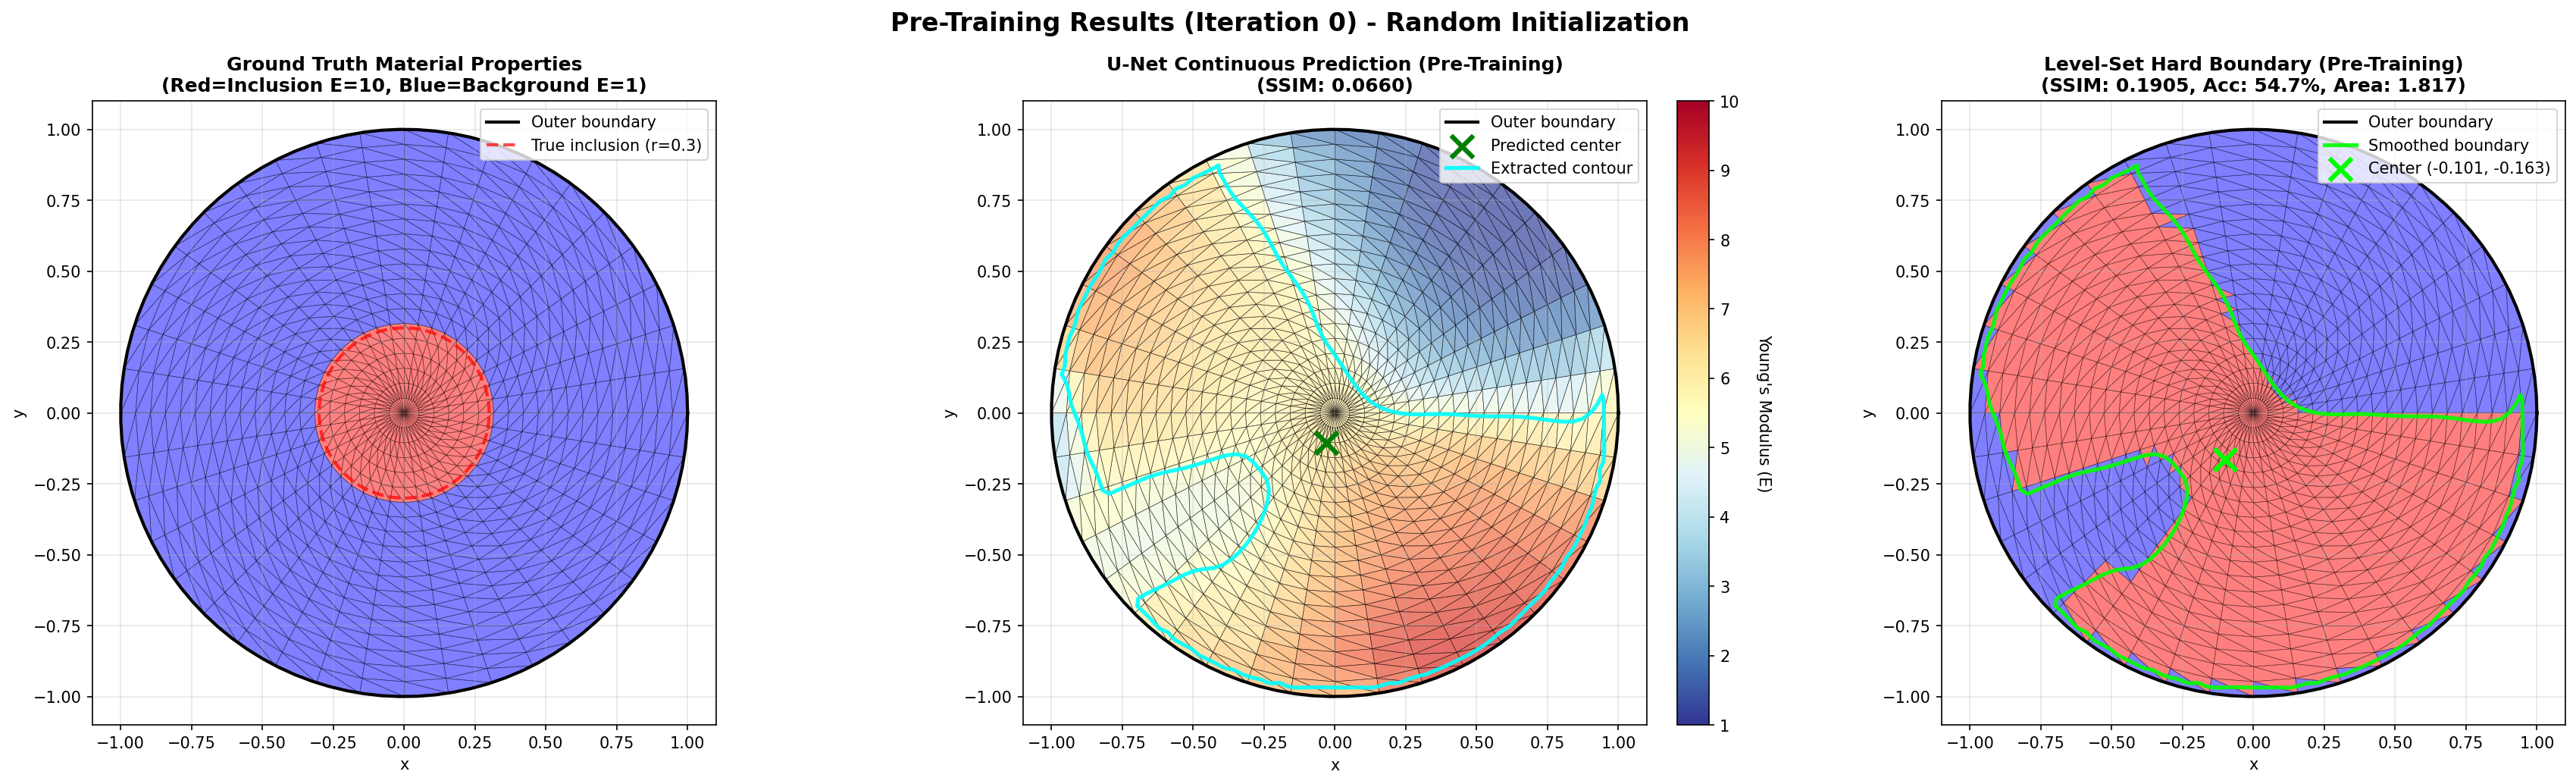
\includegraphics[width=\textwidth]{figures/pre_training_visualization.png}
\caption{Pre-training state (iteration 0) with random U-Net initialization. Left: ground truth material distribution with circular inclusion (red, $E = 10$) in background (blue, $E = 1$). Center: U-Net continuous prediction showing random material assignment (SSIM $\approx 0.06$). Right: level-set hard boundary extraction from the random prediction, bearing no resemblance to the true inclusion.}
\label{fig:pre_training}
\end{figure}

After 1000 training iterations using only the L2 displacement loss (no regularization), the network achieves an SSIM of 0.72 and pixel-wise accuracy of 87.8\%. The predicted mask captures the approximate location and size of the inclusion but exhibits diffuse boundaries and spatial noise in the material prediction. This baseline establishes that the boundary-only displacement data contains sufficient information for the U-Net to localize the inclusion through the differentiable FEM pipeline, even with the simplest possible loss function.

\begin{figure}[h!]
\centering
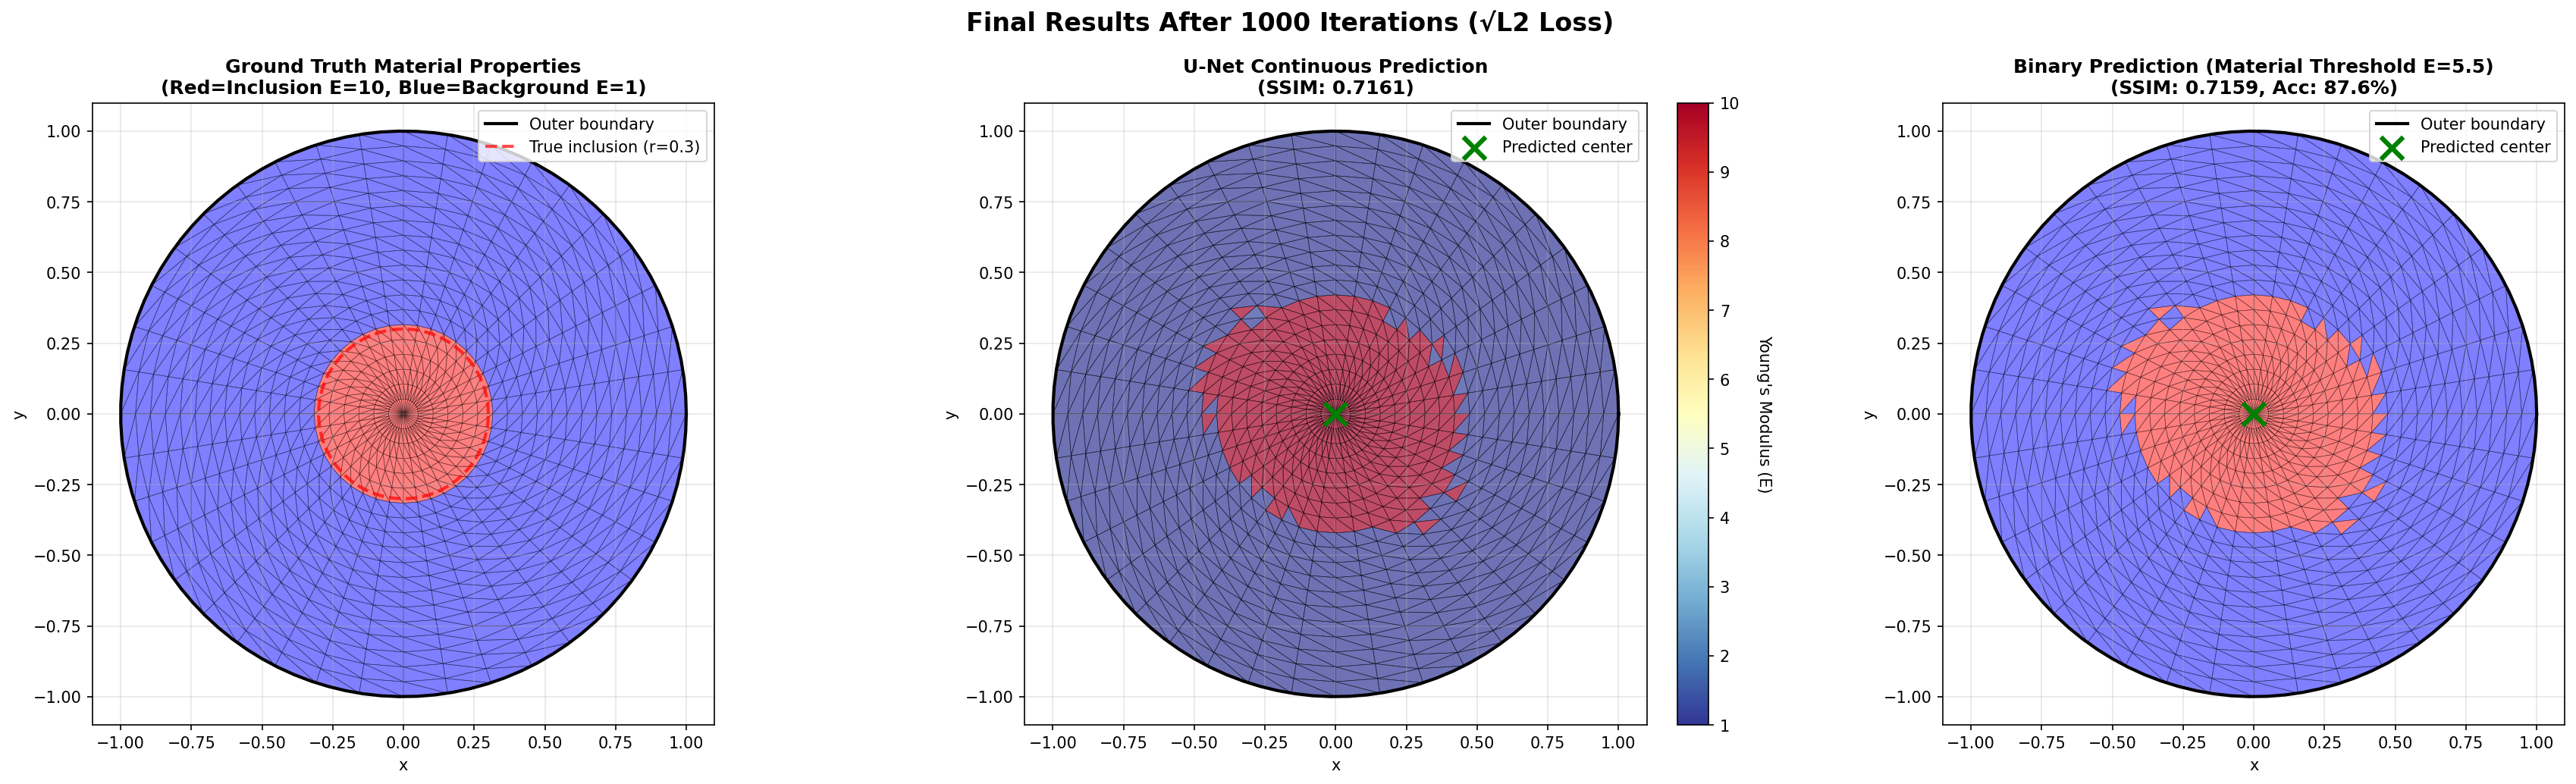
\includegraphics[width=\textwidth]{figures/vanilla_results.png}
\caption{Baseline reconstruction after 1000 iterations using only L2 displacement loss (no regularization). The U-Net localizes the inclusion (SSIM = 0.72, accuracy = 87.8\%) but the predicted boundary is diffuse with spatial noise, demonstrating the need for regularization.}
\label{fig:vanilla}
\end{figure}

Adding total variation regularization and Gaussian smoothing to the pipeline substantially improves reconstruction quality. With the composite loss $\mathcal{L} = \mathcal{L}_{\text{MSE}} + \lambda_{\text{TV}} \mathcal{L}_{\text{TV}}$ and level-set post-processing, the SSIM increases to 0.91 with 94.6\% accuracy after 1000 iterations. The predicted inclusion boundary becomes crisp and closely matches the ground truth circular geometry. This improvement confirms that TV regularization serves its intended purpose: promoting the piecewise constant material distributions that the segmentation formulation assumes.

\begin{figure}[h!]
\centering
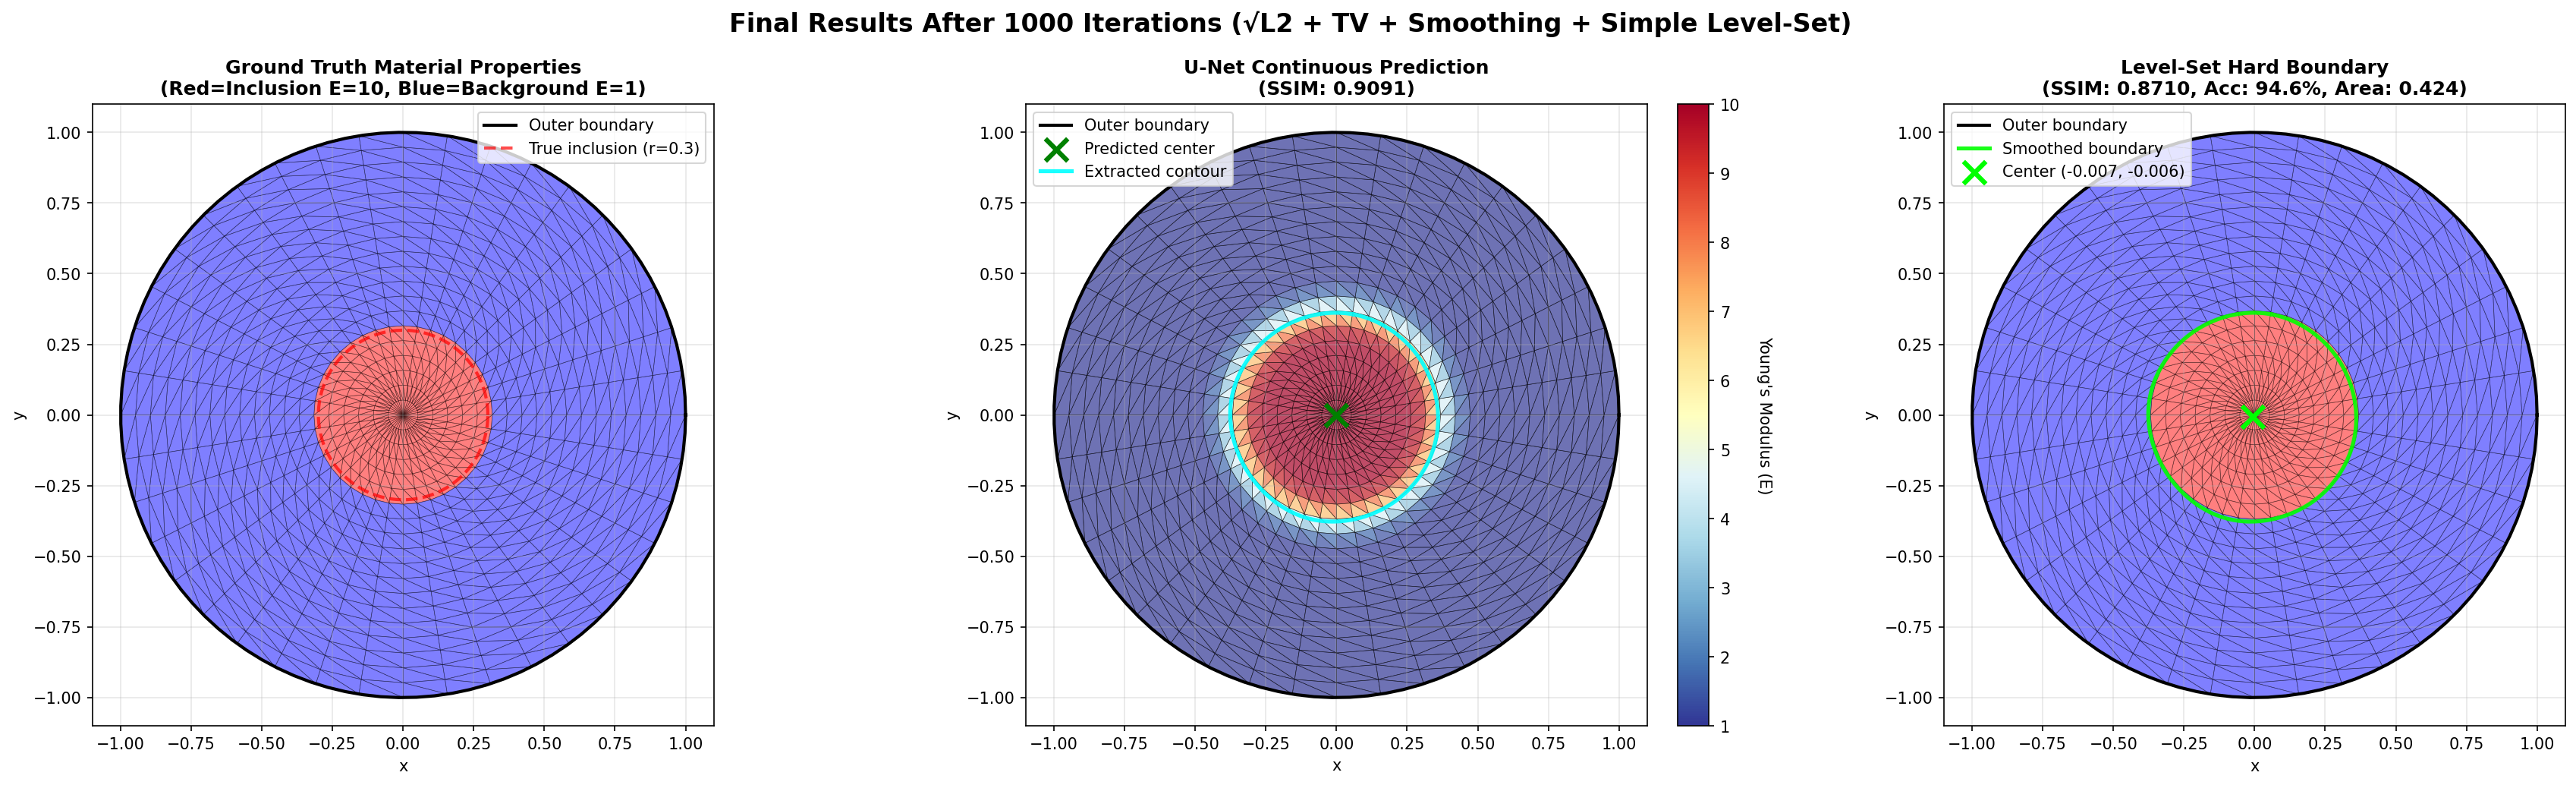
\includegraphics[width=\textwidth]{figures/post_training_visualization.png}
\caption{Reconstruction with TV regularization, Gaussian smoothing, and level-set post-processing after 1000 iterations (SSIM = 0.91, accuracy = 94.6\%). The predicted inclusion boundary is crisp and closely matches the ground truth circular geometry, confirming the effectiveness of the composite loss function.}
\label{fig:post_training_full}
\end{figure}

\subsection*{Grid Search Optimization}

Systematic hyperparameter tuning via grid search over learning rate, TV weight $\lambda_{\text{TV}}$, smoothing kernel width $\sigma$, thresholding temperature $T$, and boundary condition sharpness yields further improvement in efficiency. The optimized configuration achieves an SSIM of 0.85 with 94.6\% accuracy in only 200 iterations---a five-fold reduction in iterations compared to the untuned baseline at comparable reconstruction quality. This demonstrates that the algorithm's performance is sensitive to hyperparameter selection and that systematic tuning is essential for practical deployment.

\begin{figure}[h!]
\centering
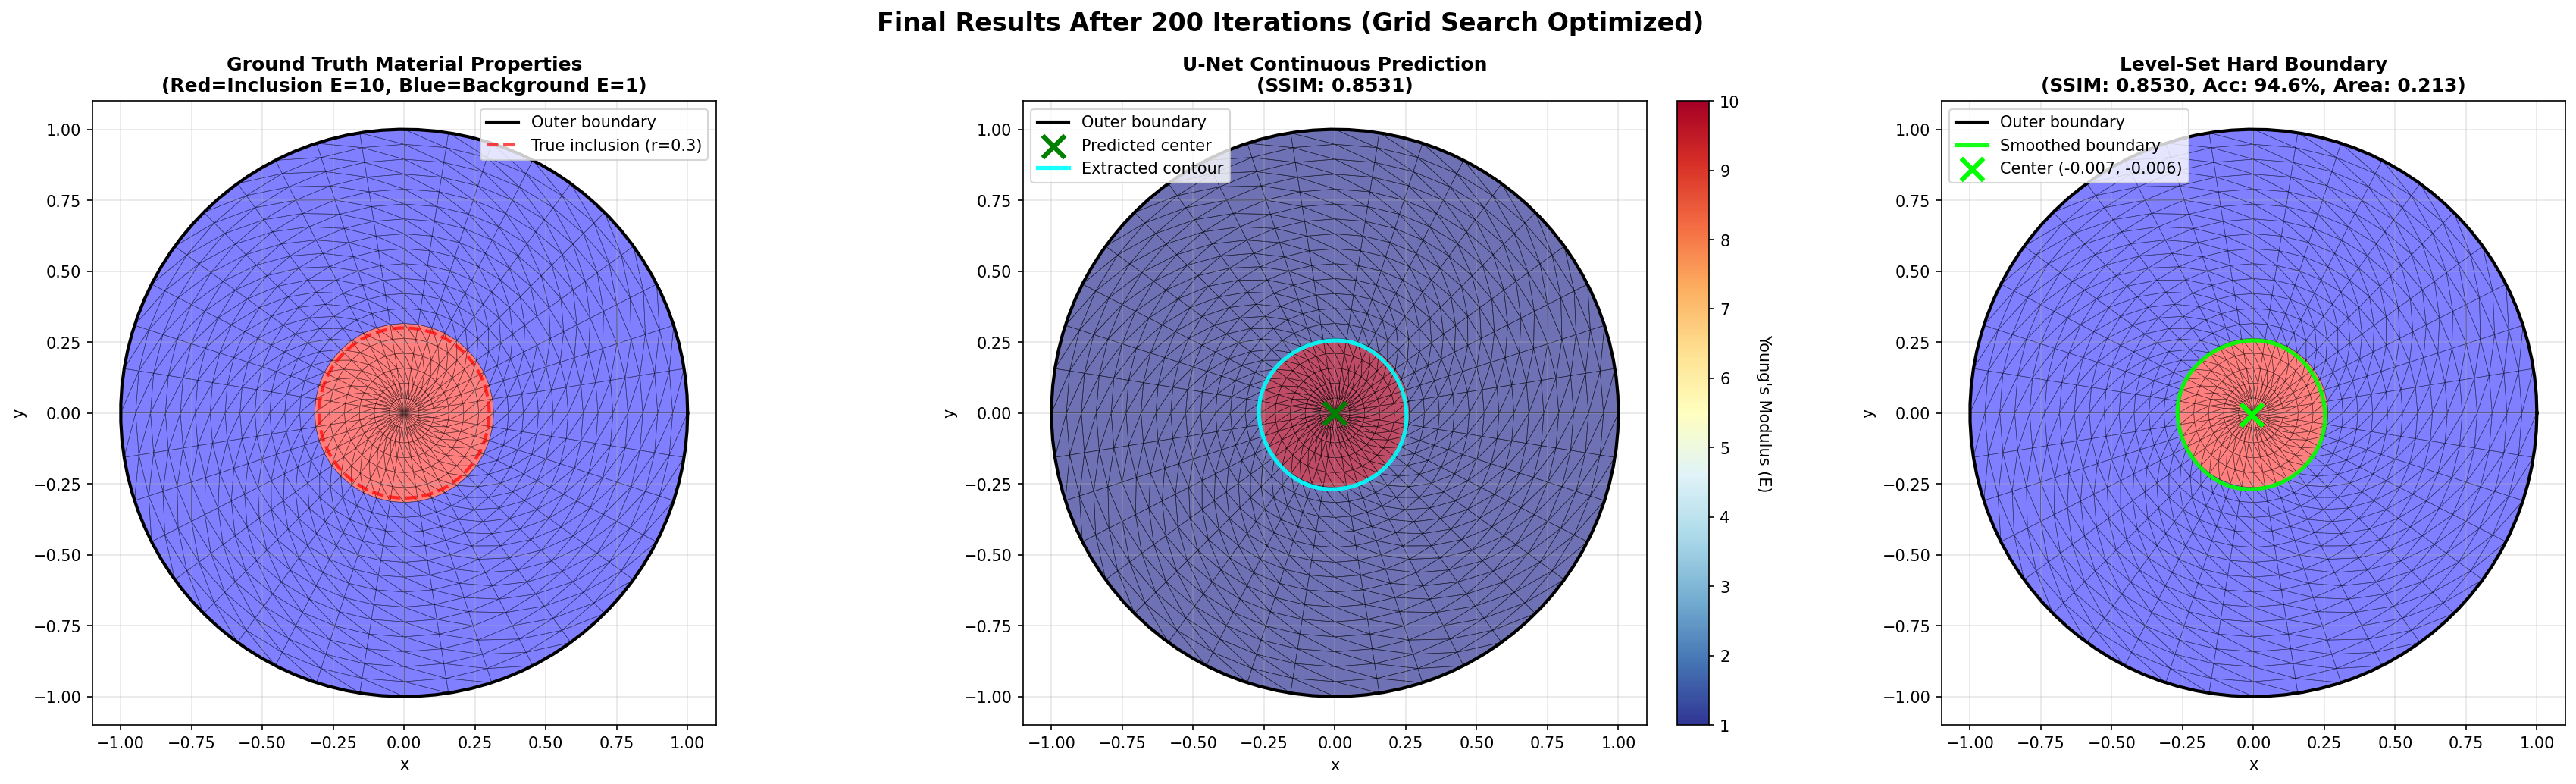
\includegraphics[width=\textwidth]{figures/post_training_visualization_grid_search_optimized.png}
\caption{Grid-search-optimized reconstruction after only 200 iterations (SSIM = 0.85, accuracy = 94.6\%). Systematic hyperparameter tuning achieves comparable accuracy to the untuned result (Figure~\ref{fig:post_training_full}) in one-fifth the iterations.}
\label{fig:grid_search}
\end{figure}

\subsection*{Challenging Scenarios: Faint and Small Inclusions}

To probe the limits of the methodology, we tested three progressively more challenging scenarios using the grid-search-optimized hyperparameters.

For a faint inclusion with low stiffness contrast ($\alpha = 1.2$, compared to the standard $\alpha = 10$), the algorithm achieves an SSIM of 0.81 with 93.0\% accuracy. Despite the subtle displacement differences produced by a near-background-stiffness inclusion, the method successfully detects and localizes the inclusion. The reconstruction quality degrades gracefully relative to the high-contrast case.

\begin{figure}[h!]
\centering
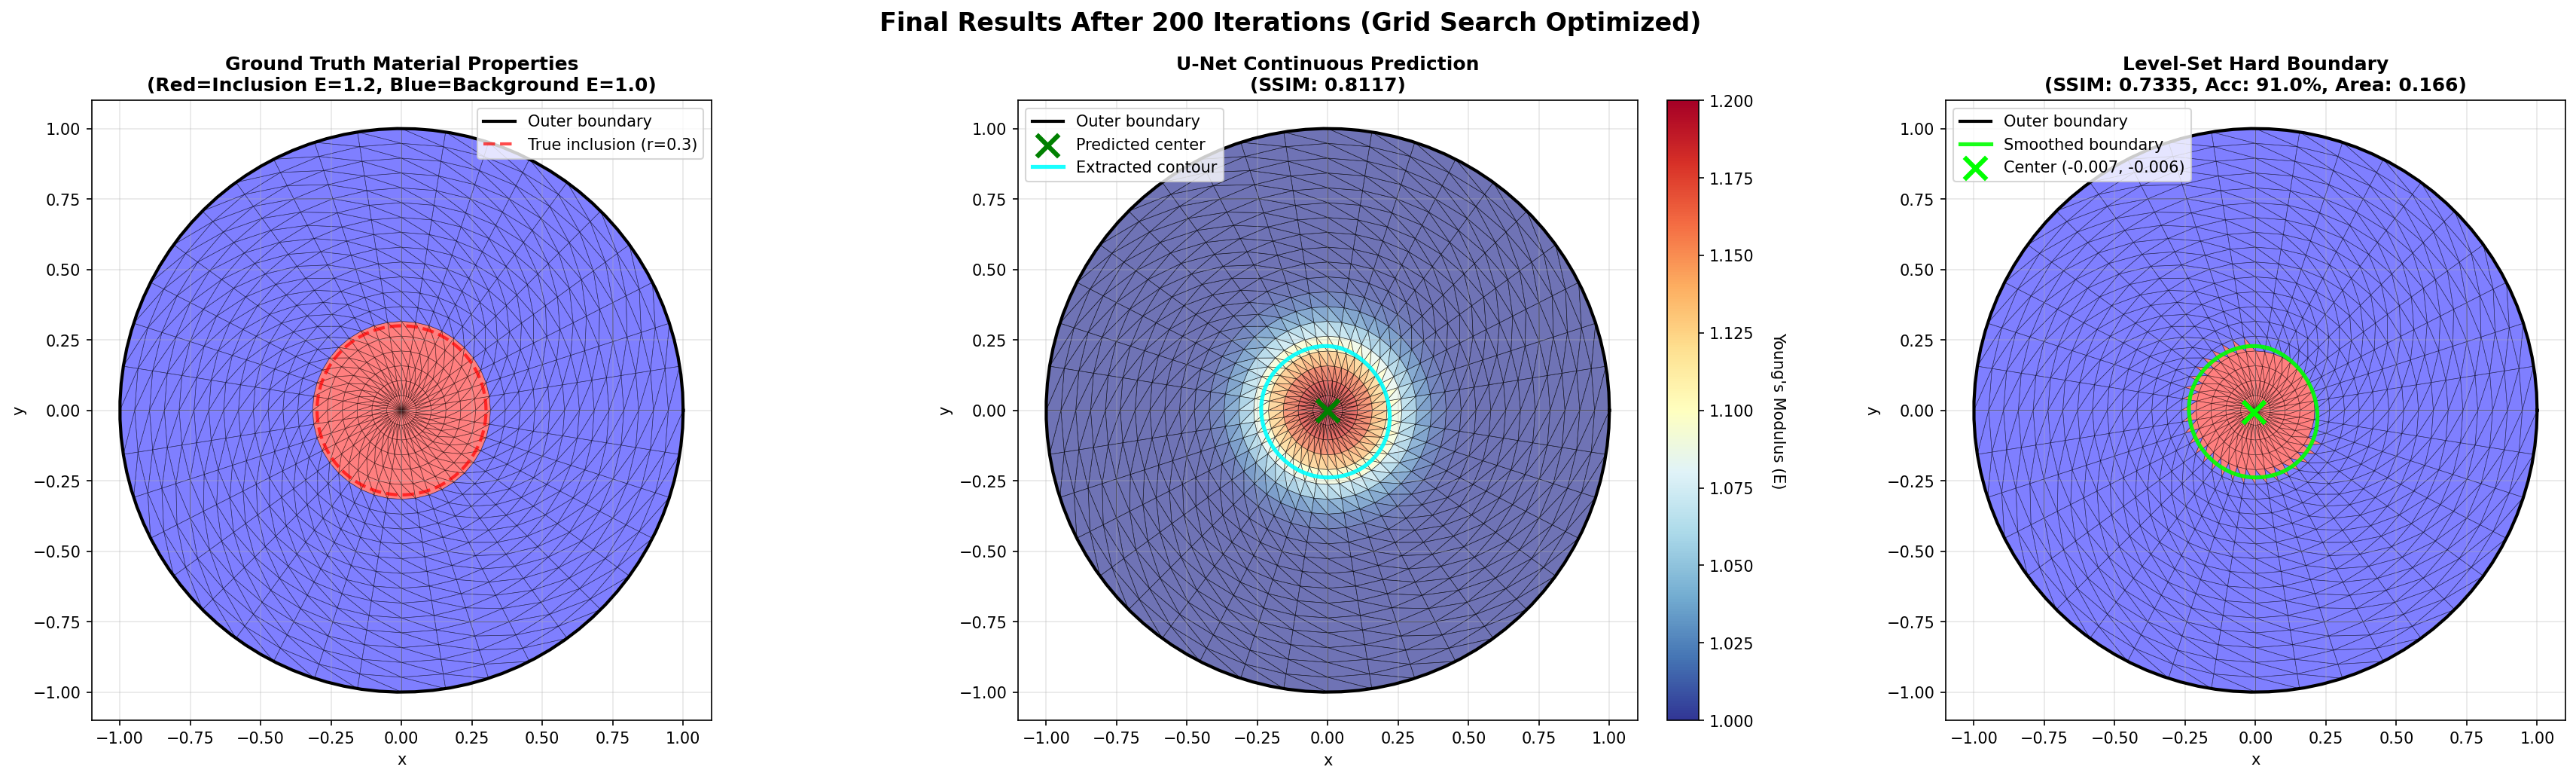
\includegraphics[width=\textwidth]{figures/post_training_visualization_grid_search_optimized_faint_inclusion.png}
\caption{Faint inclusion reconstruction ($\alpha = 1.2$, SSIM = 0.81, accuracy = 93.0\%). Despite the low stiffness contrast producing subtle boundary displacement differences, the method successfully detects and localizes the inclusion with graceful quality degradation.}
\label{fig:faint}
\end{figure}

For a smaller inclusion with reduced radius, the algorithm achieves an SSIM of 0.40 with 88.5\% accuracy. The inclusion location is correctly identified, but the boundary geometry is less precisely recovered. Small inclusions produce weaker displacement signals at the boundary, reducing the information available for reconstruction.

\begin{figure}[h!]
\centering
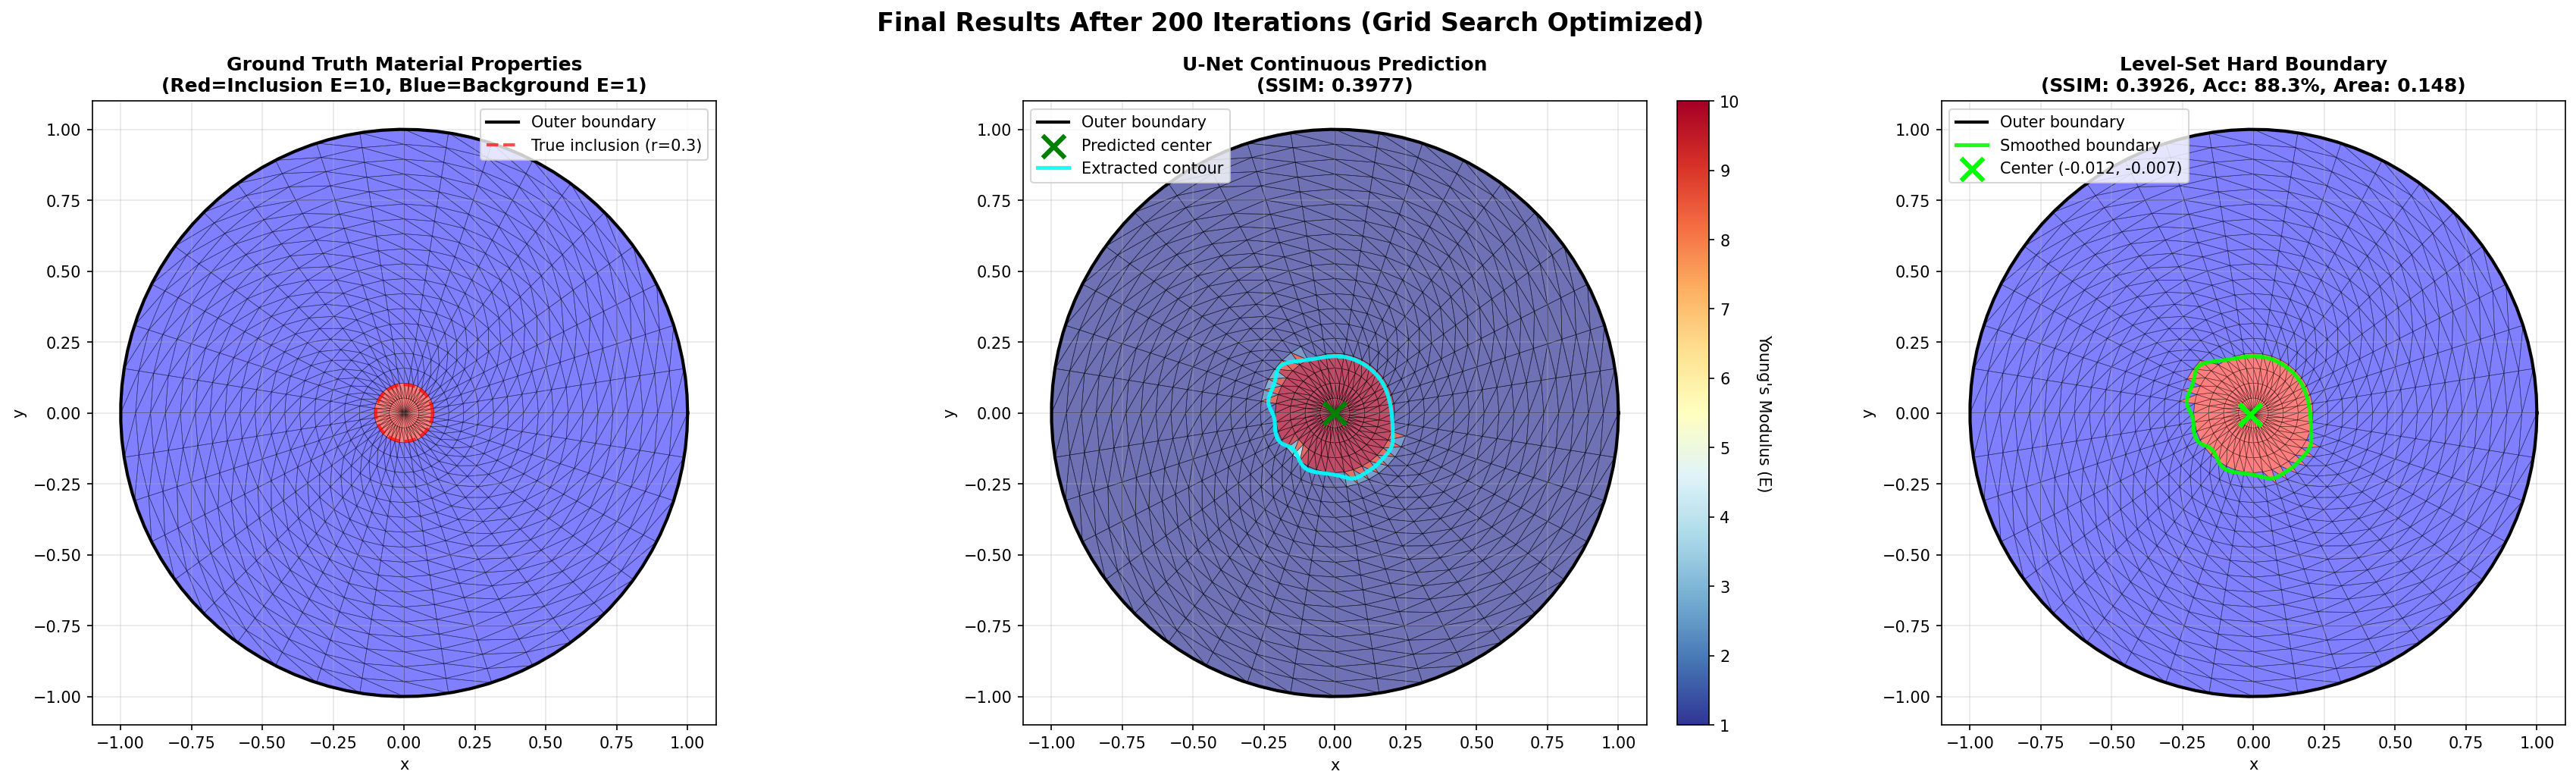
\includegraphics[width=\textwidth]{figures/post_training_visualization_grid_search_optimized_smaller_inclusion.png}
\caption{Smaller inclusion reconstruction (SSIM = 0.40, accuracy = 88.5\%). The inclusion location is correctly identified, but boundary geometry is less precisely recovered due to the weaker displacement signal produced by the reduced inclusion size.}
\label{fig:smaller}
\end{figure}

The most challenging scenario combines both difficulties: a small inclusion with faint contrast ($\alpha = 1.2$). Here the algorithm achieves an SSIM of 0.49 with 89.5\% accuracy. The inclusion is still detected and approximately localized, but reconstruction fidelity is reduced. This case represents a fundamental sensitivity limit where the displacement signal from the inclusion approaches the numerical precision of the solver.

\begin{figure}[h!]
\centering
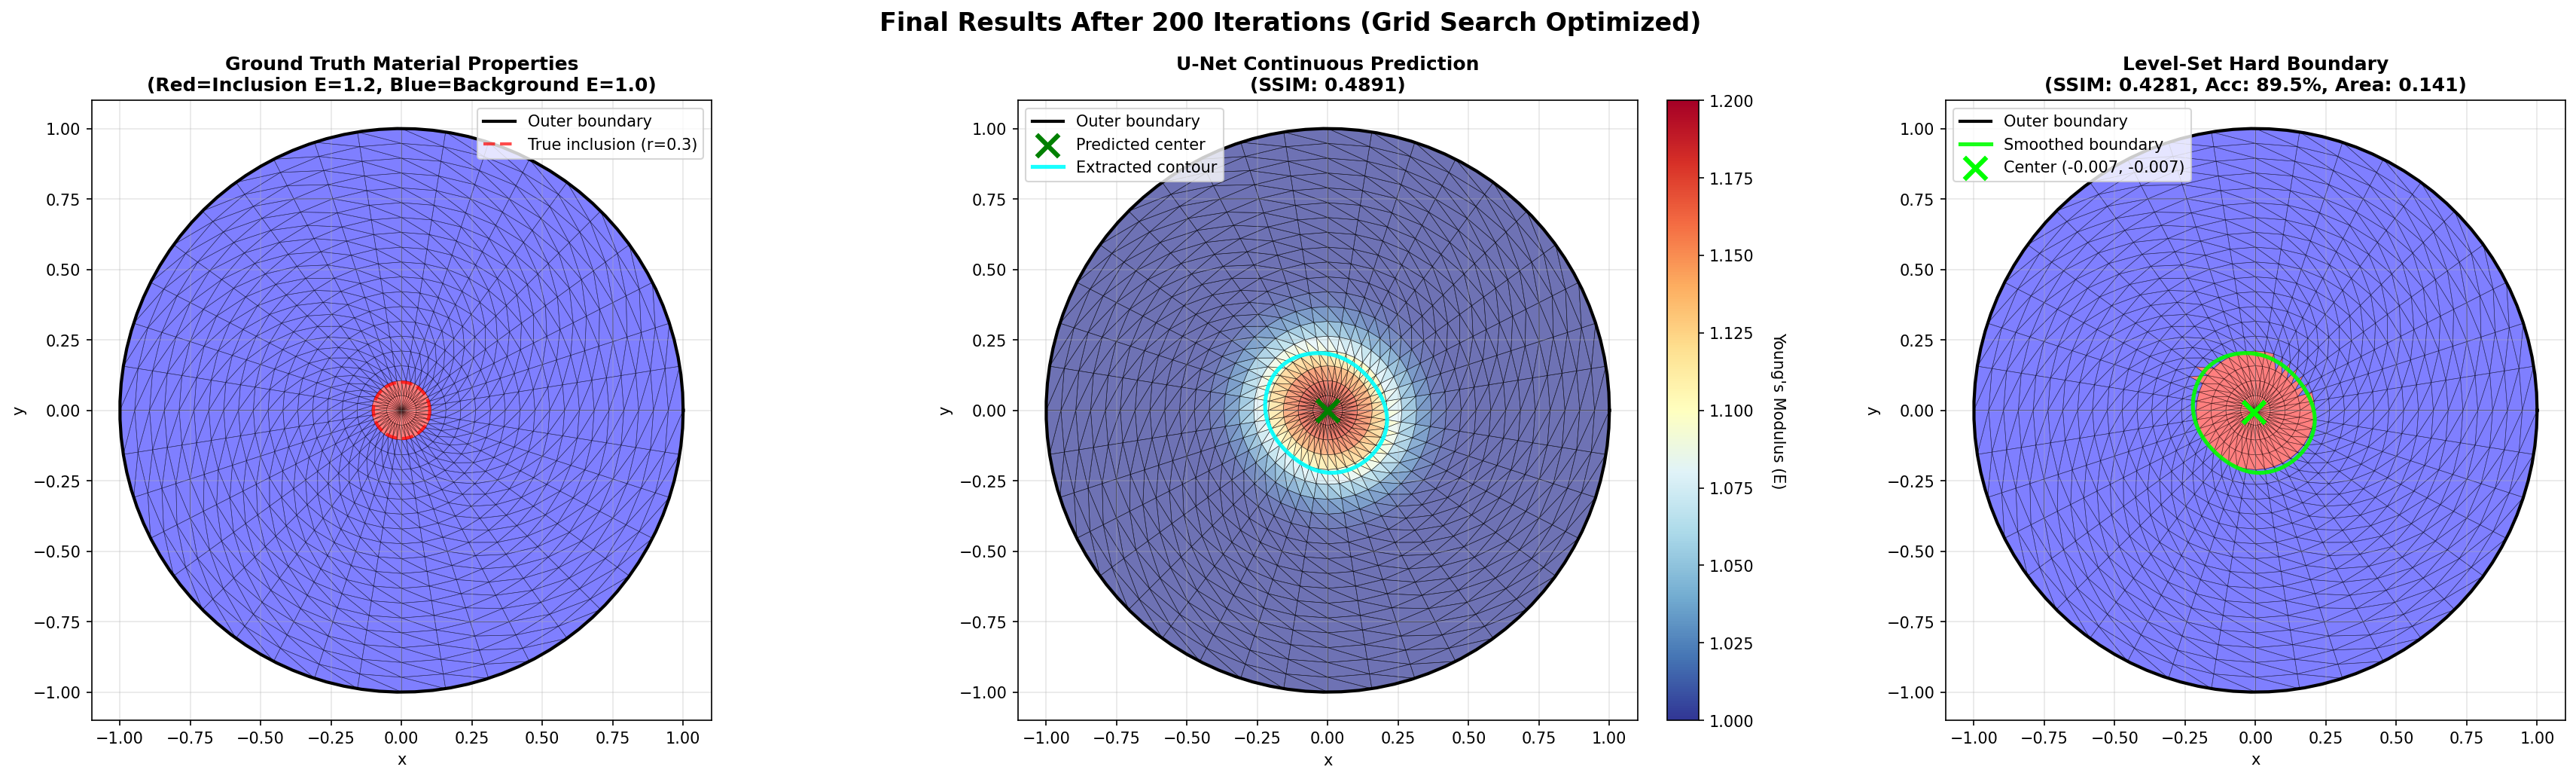
\includegraphics[width=\textwidth]{figures/post_training_visualization_grid_search_optimized_small_and_faint_inclusion.png}
\caption{Most challenging scenario: small inclusion with faint contrast ($\alpha = 1.2$, SSIM = 0.49, accuracy = 89.5\%). The inclusion is detected and approximately localized, representing the sensitivity limit of the current methodology.}
\label{fig:small_faint}
\end{figure}

These results establish a performance envelope: the method works well for standard clinical contrast ratios ($\alpha \geq 5$) and medium-to-large inclusions, with graceful degradation as either contrast or size decreases.

\subsection*{Robustness to Initialization: Reliability Study}

A critical concern for any optimization-based reconstruction method is sensitivity to random weight initialization. To assess this, we conducted a reliability study consisting of multiple independent runs with identical training procedures, hyperparameters, and datasets, varying only the random seed for U-Net weight initialization.

\begin{figure}[h!]
\centering
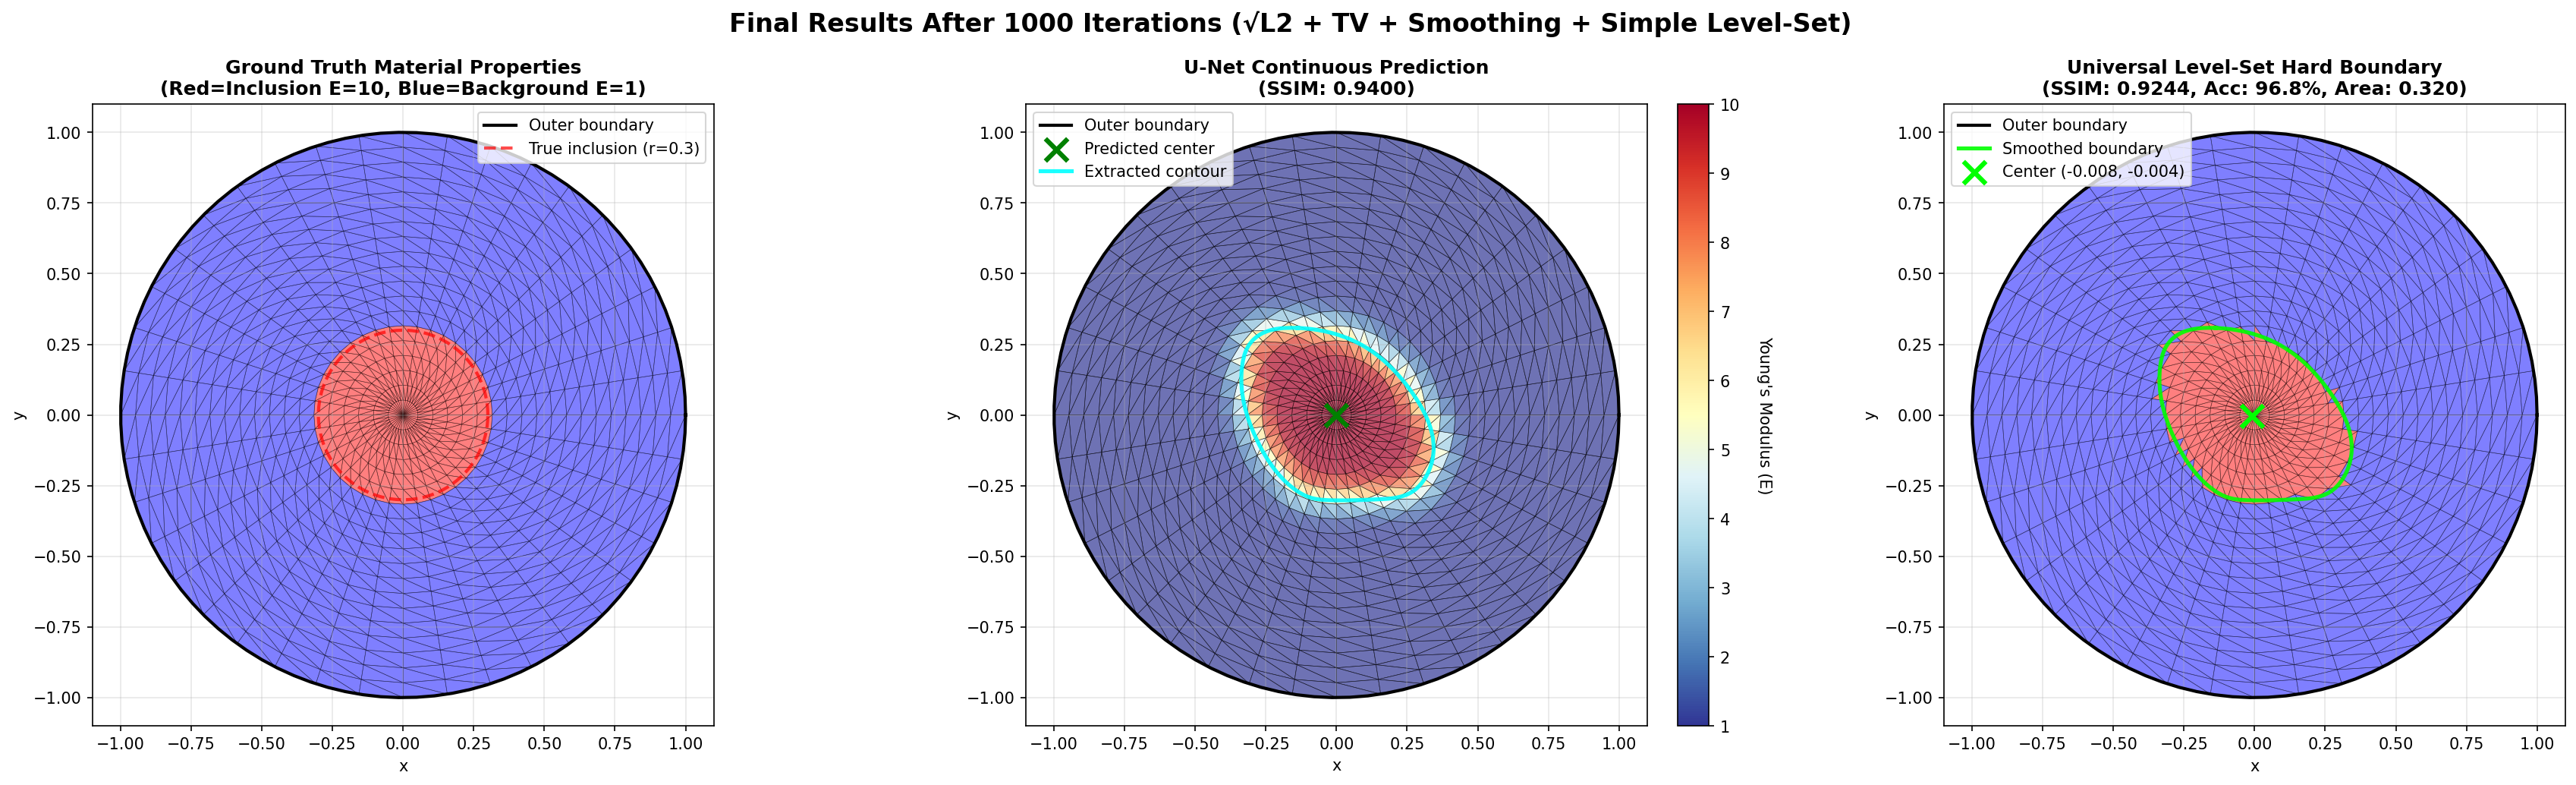
\includegraphics[width=\textwidth]{figures/sensitivity_to_initial_conditions.png}
\caption{Robustness to initialization demonstrated across multiple independent runs. Each run uses identical training procedure and data with different random seeds. The reconstructions achieve consistent SSIM values above 0.90 with visually similar inclusion boundaries, confirming that the optimizer converges to the same solution regardless of initialization.}
\label{fig:sensitivity}
\end{figure}

The results demonstrate tight clustering across runs. Individual reconstructions achieve SSIM values consistently above 0.90 with accuracy above 93\%, and the predicted inclusion boundaries are visually similar across all runs. No spurious local minima were observed---every run converged to a high-quality reconstruction. This tight clustering confirms that the combination of angular and symmetric scanning data provides sufficient constraints to guide the optimizer toward consistent solutions regardless of initialization, validating the robustness claims made for the symmetric scanning innovation.

\begin{figure}[h!]
\centering
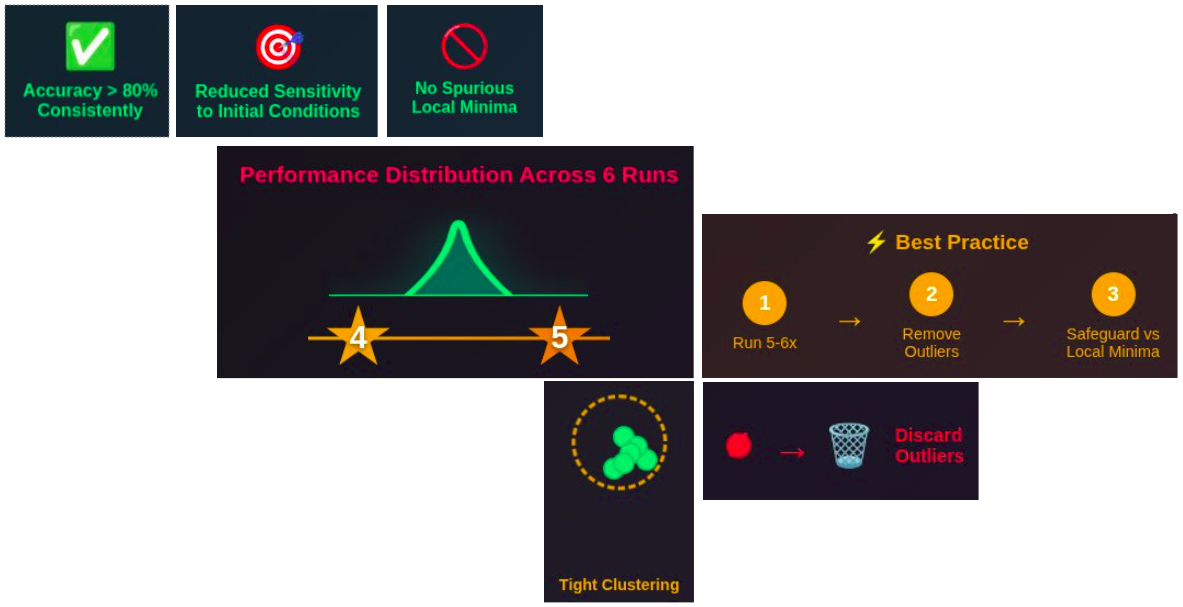
\includegraphics[width=0.9\textwidth]{figures/reliability_study_poc_pat_scan.png}
\caption{Summary of reliability study findings: accuracy consistently above 80\%, reduced sensitivity to initial conditions, and no spurious local minima. The tight clustering across runs motivates a practical ensemble strategy where the practitioner runs the algorithm 3--5 times, discards outliers, and averages the clustered results.}
\label{fig:reliability_summary}
\end{figure}

\subsection*{Extension to Irregular Geometry}

As an initial test of generalizability beyond the proof-of-concept circular geometry, we applied the methodology to an irregular, off-centered inclusion parameterized by Fourier series boundary perturbations. This represents a significantly harder reconstruction task: the inclusion boundary is non-convex with complex geometric features, and the off-center placement breaks the rotational symmetry exploited by symmetric scanning.

An initial attempt without learning rate optimization achieved an SSIM of only 0.21 after 600 iterations (approximately 13 minutes of computation), failing to capture the irregular boundary shape.

\begin{figure}[h!]
\centering
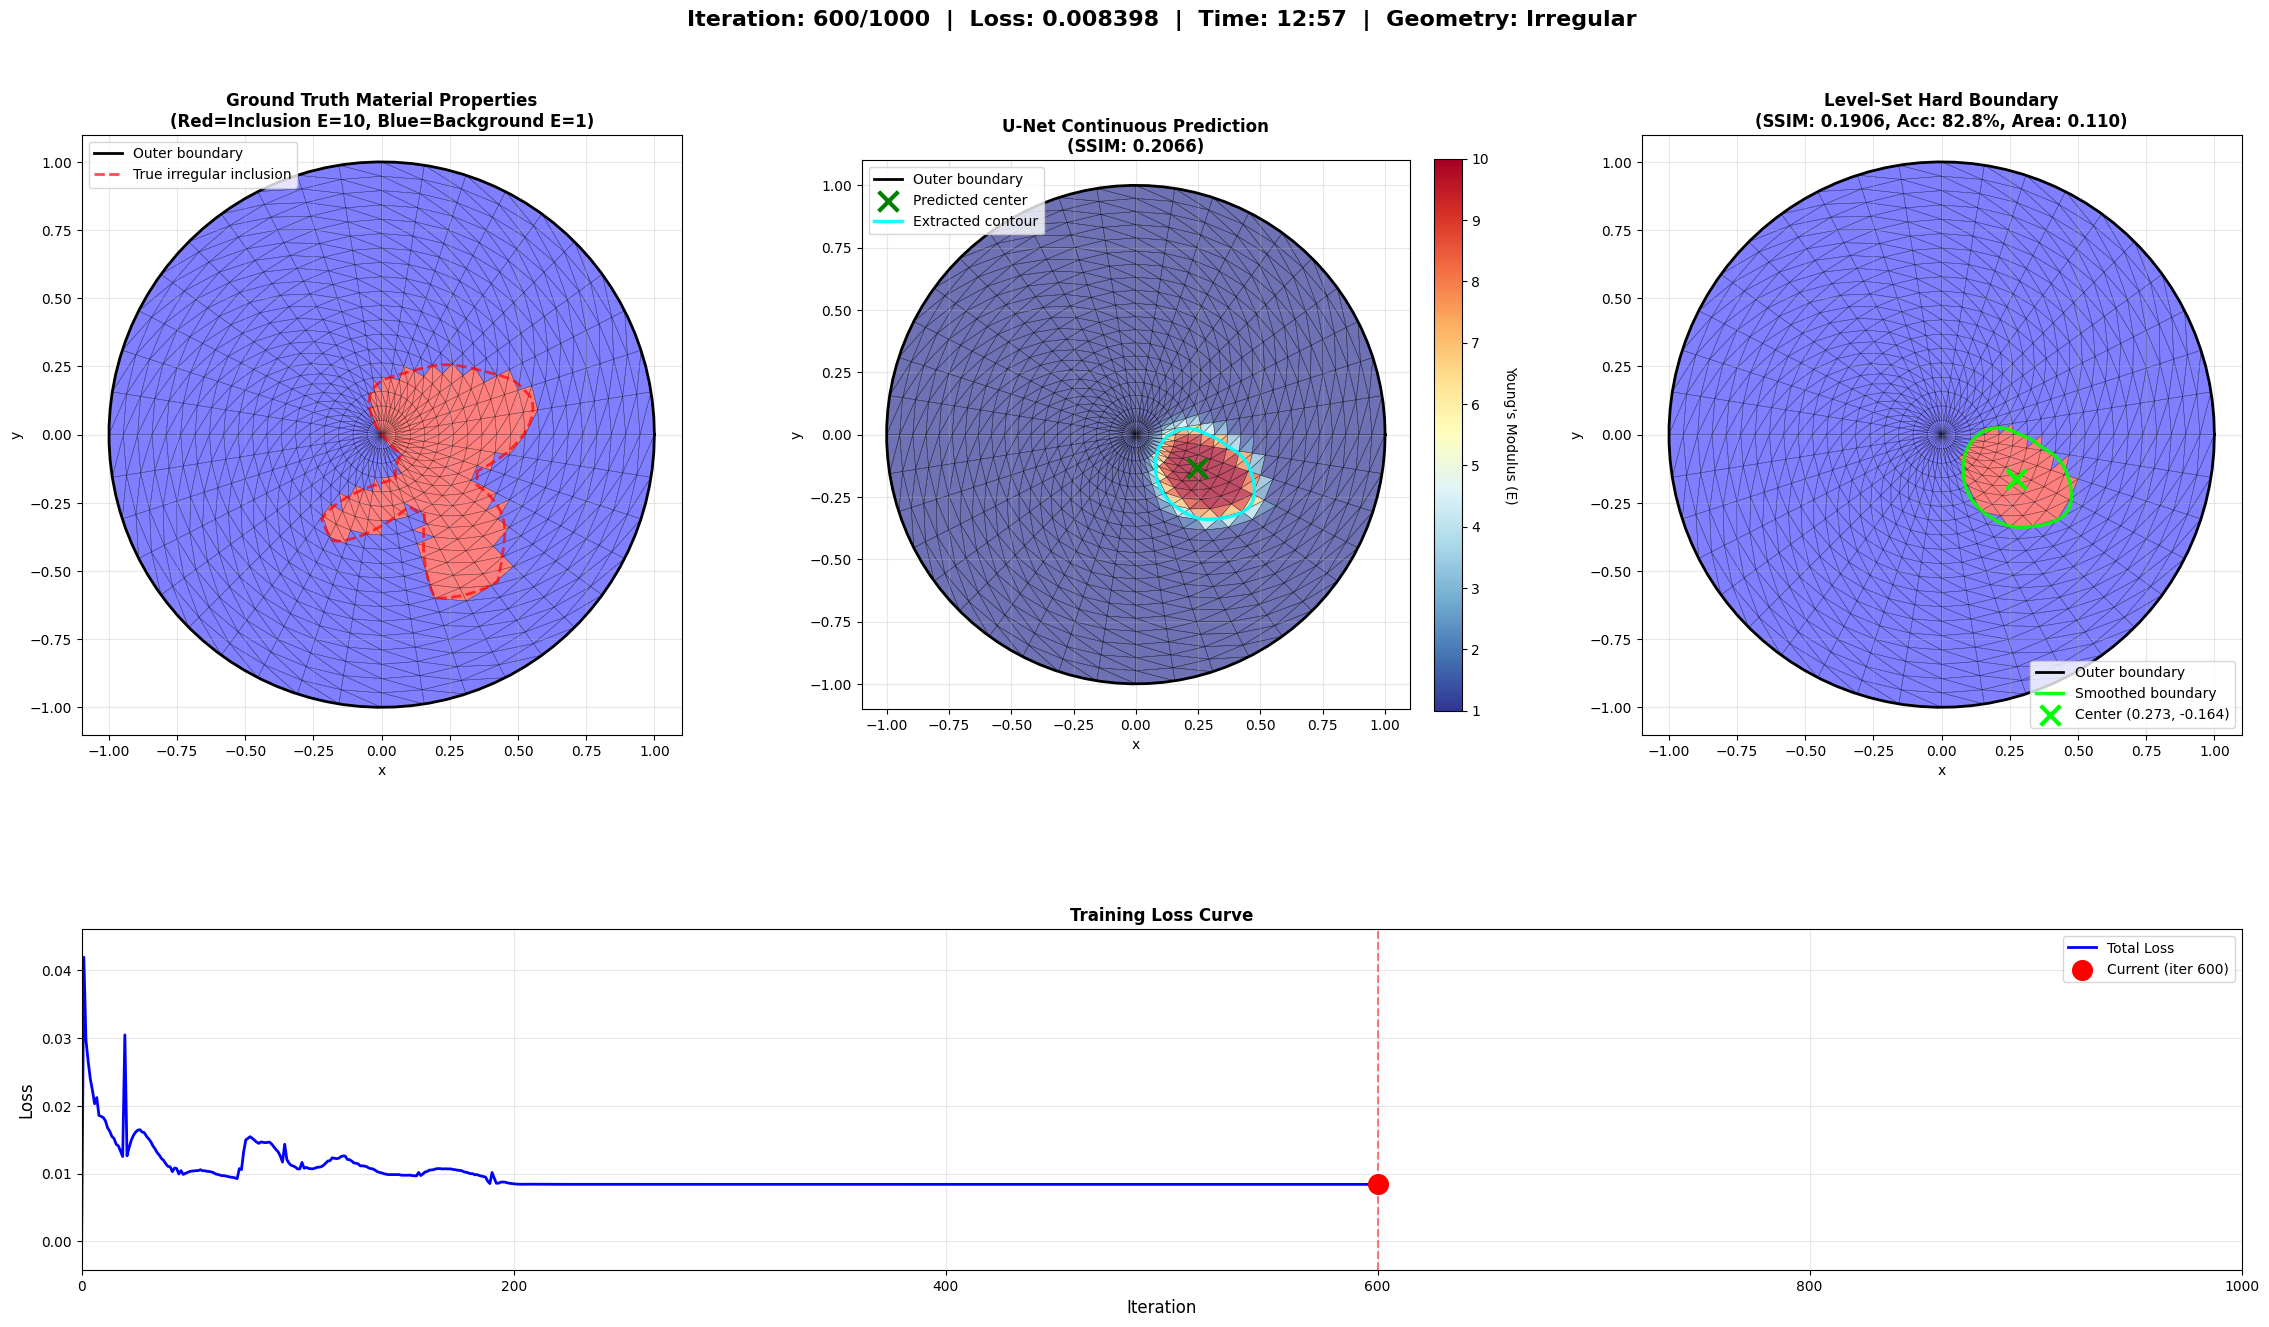
\includegraphics[width=\textwidth]{figures/irregular_inclusion_preliminary_results.png}
\caption{Irregular inclusion reconstruction without learning rate optimization (SSIM = 0.21, approximately 13 minutes). The reconstruction fails to capture the complex boundary shape, highlighting the sensitivity of irregular geometries to hyperparameter selection. The training loss curve (bottom) shows convergence but to a poor local minimum.}
\label{fig:irregular_no_lr}
\end{figure}

After including learning rate in the hyperparameter grid search, reconstruction quality improved dramatically to an SSIM of 0.80 with 92.7\% accuracy (approximately 17 minutes of computation). The predicted boundary captures the overall shape and location of the irregular inclusion, though fine geometric detail is smoothed. The loss curve shows stable convergence without oscillation.

\begin{figure}[h!]
\centering
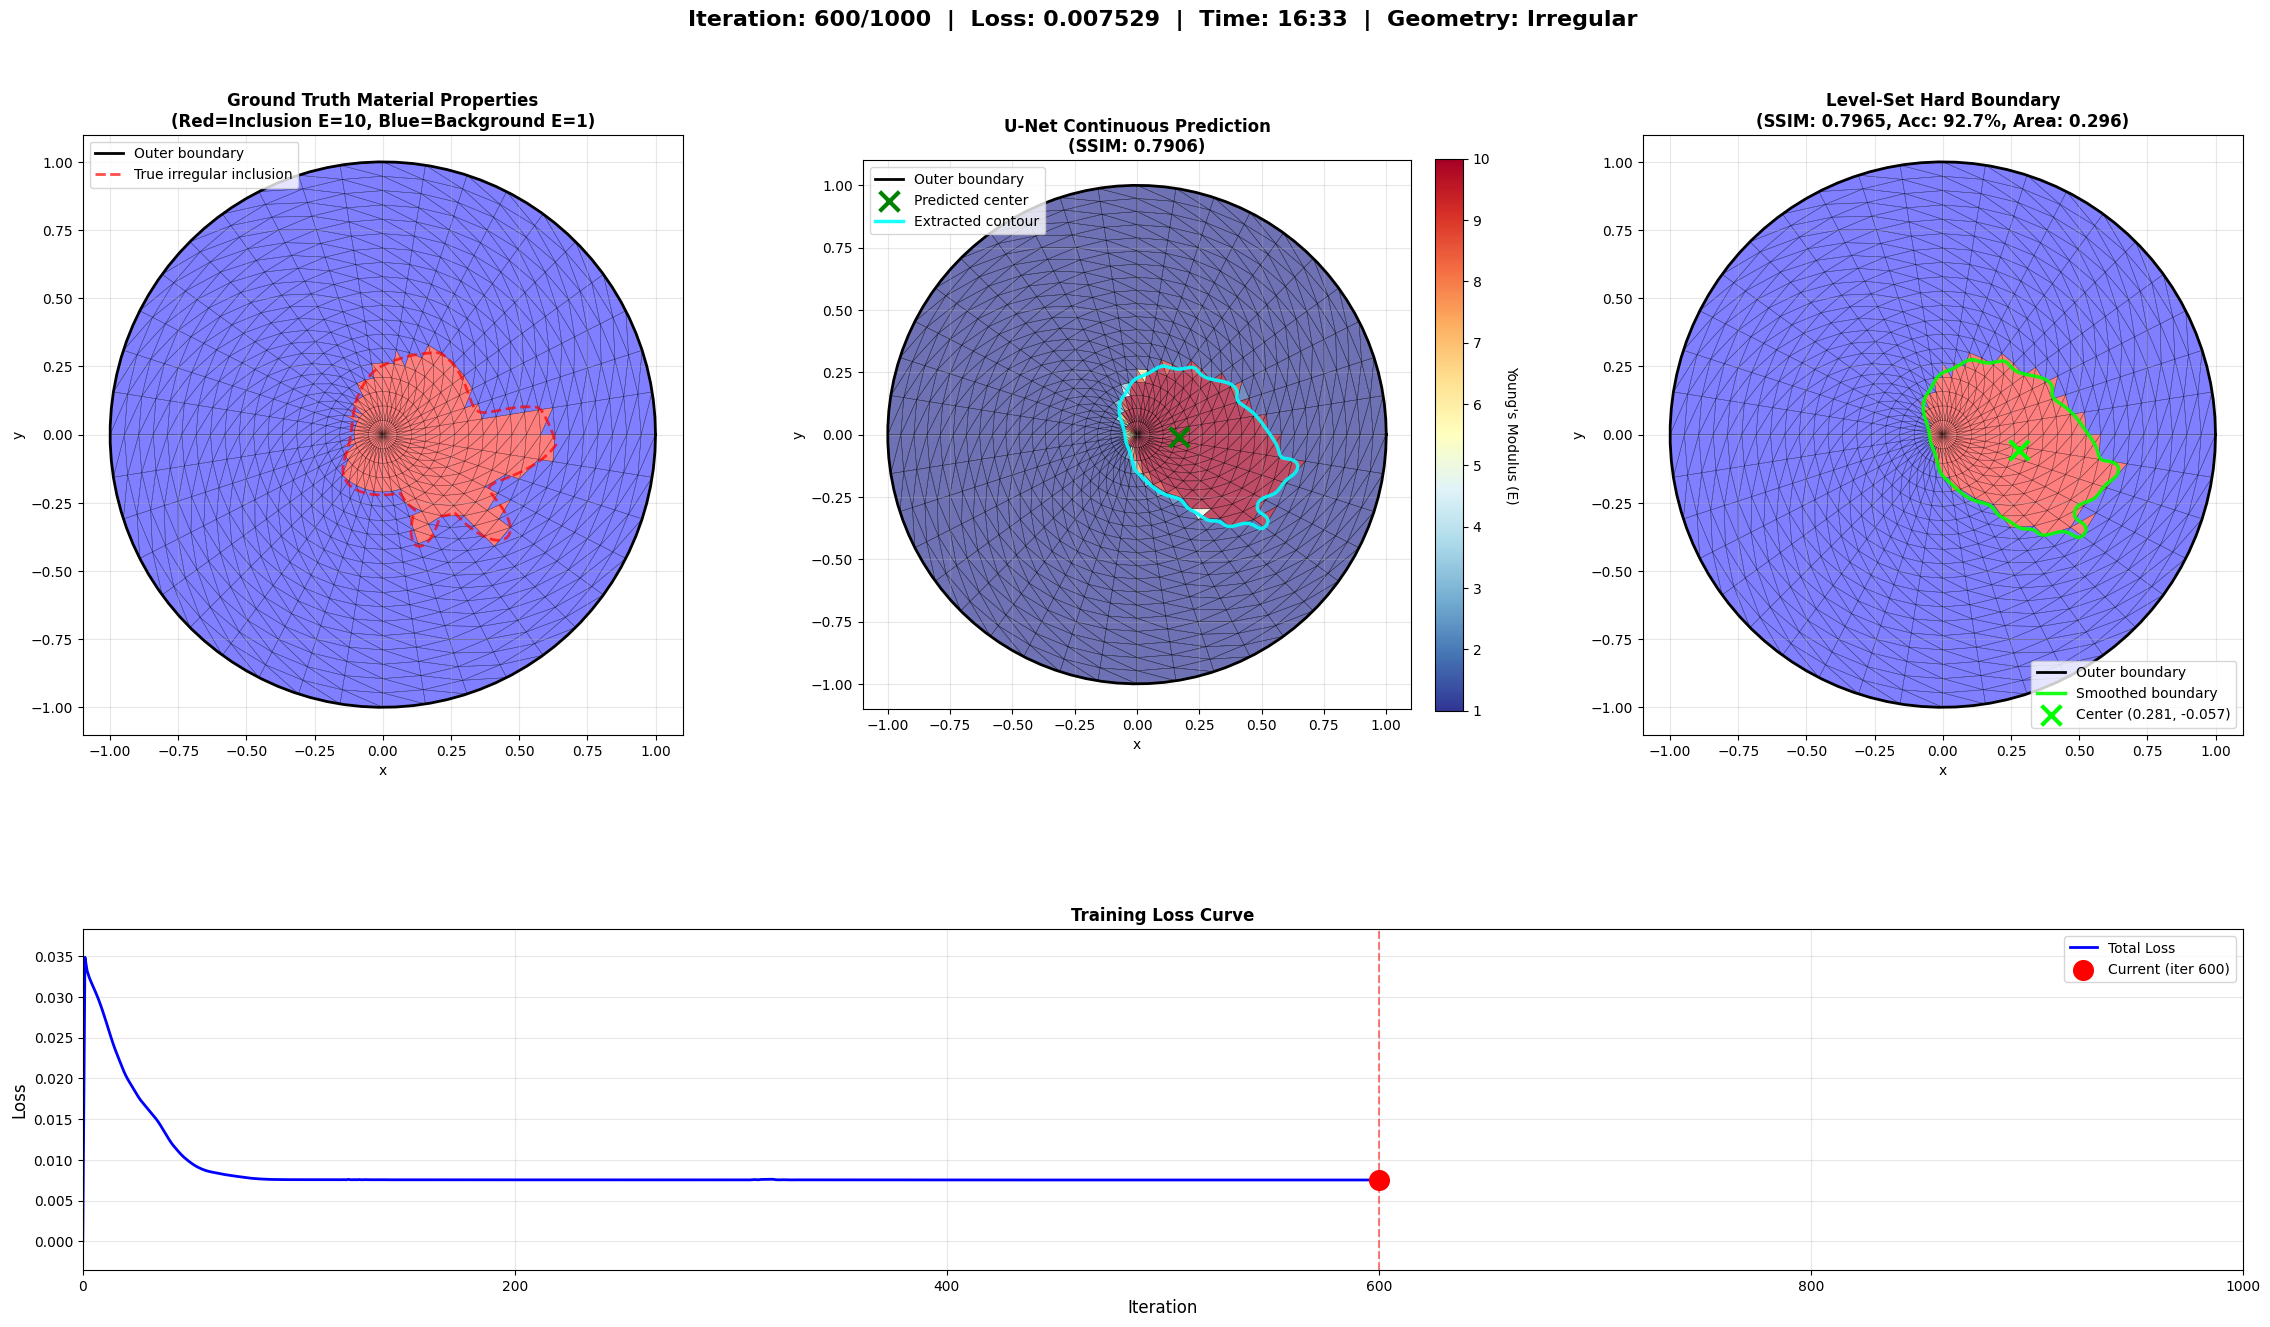
\includegraphics[width=\textwidth]{figures/irregular_inclusion_learning_rate_optimized.png}
\caption{Irregular inclusion reconstruction with learning rate optimization (SSIM = 0.80, accuracy = 92.7\%, approximately 17 minutes). The same U-Net architecture generalizes to non-convex, off-centered inclusion geometry without architectural modifications. The predicted boundary captures the overall shape and location, with the loss curve (bottom) showing stable convergence.}
\label{fig:irregular_lr}
\end{figure}

This preliminary result on irregular geometry demonstrates that the same U-Net architecture generalizes beyond the idealized circular case without architectural modifications, while highlighting the importance of hyperparameter optimization---particularly learning rate selection---for more complex geometries. Full systematic evaluation of irregular inclusions is the subject of Specific Aim 2a.

\subsection*{Summary of Preliminary Findings}

These preliminary results establish several key findings. First, boundary-only displacement measurements contain sufficient information for inclusion reconstruction, validating the core premise of PAT Scan. Second, the segmentation-based formulation with U-Net successfully recovers inclusion geometry from the differentiable FEM pipeline. Third, total variation regularization and systematic hyperparameter tuning are essential for high-quality reconstruction. Fourth, the method is robust to random initialization, producing consistent results across independent runs. Fifth, the approach generalizes to irregular geometries with appropriate hyperparameter selection. These findings provide the foundation for the systematic research program described in the following section.

\newpage

% Section E: Research Approach
% Auto-generated from comps_skeleton_vivek-equations-extracted.md
% Zero-deletion protocol: all prose preserved exactly

\section*{E. Research Approach}

The research strategy follows a natural progression from simplified proof-of-concept to realistic complexity, systematically addressing key challenges at each stage. This approach mirrors the development trajectory of successful imaging technologies: establish feasibility on idealized cases, then progressively incorporate real-world complexity until clinical translation becomes viable.

The overarching goal of this research is to improve understanding of the PAT Scan methodology for tissue stiffness reconstruction through systematic development. This goal unfolds across three specific aims that build upon one another in a deliberate arc. Specific Aim 1 establishes a proof-of-concept with circular geometries, demonstrating that the fundamental approach is sound. Specific Aim 2 extends the methodology to realistic complexity within the 2D domain, confronting the irregular shapes, heterogeneous materials, and optimized data acquisition strategies that clinical scenarios demand. Specific Aim 3 incorporates 3D geometry and clinical realism, bridging the gap between computational simulation and eventual patient care.

\subsection*{Specific Aim 1: Proof-of-Concept}

The first specific aim is to demonstrate proof-of-concept for the PAT Scan methodology by focusing on the tractable geometric inverse problem of inclusion localization, using simple 2D circular geometry for validation, and establishing that boundary displacement measurements contain sufficient information for reconstruction.

\subsubsection*{Working Assumption: Existence of Inclusion}

The methodology operates under the assumption that one singular inclusion exists within the sample. This assumption is straightforward to verify in practice through a simple four-step verification procedure. First, boundary displacement measurements are acquired under applied forces. Second, these measurements are compared to reference displacements for a homogeneous circular sample with known background Young's modulus and no inclusion. Third, if the measured displacements deviate significantly from the homogeneous reference, an inclusion is present. Fourth, if displacements match the homogeneous reference, no inclusion exists, or the inclusion has negligible contrast.

This verification step serves as a prerequisite gate before applying the PAT Scan reconstruction algorithm. The method targets scenarios where palpation or preliminary screening has already detected an abnormality; PAT Scan characterizes its geometry and stiffness quantitatively.

\subsection*{Specific Aim 1a: FEM Forward Model Development}

A standard finite element method (FEM) solver for 2D plane strain linearized elasticity is implemented. The mesh employs a structured polar grid, which naturally suits circular and near-circular geometries while providing efficient triangulation.

\subsubsection*{Mathematical Formulation}

The governing equations rest on linearized elasticity for small deformations under quasi-static loading where inertia and damping are neglected. The fundamental relationship is captured by the static equilibrium equation

\begin{equation*}
\mathbf{F} = \mathbf{K} \mathbf{U}
\end{equation*}

where $\mathbf{F}$ is the applied force vector of dimension $n_{\text{dof}} \times 1$, $\mathbf{K}$ is the global stiffness matrix of dimension $n_{\text{dof}} \times n_{\text{dof}}$, and $\mathbf{U}$ is the displacement vector of dimension $n_{\text{dof}} \times 1$. A plane stress assumption is adopted, setting the out-of-plane stress component to zero, which is appropriate for thin samples.

The material properties are specified as follows. Young's modulus $E(x, y)$ is piecewise constant, with the background modulus normalized to $E_{\text{bg}} = 1.0$ in normalized units. The inclusion modulus varies according to a multiplicative contrast factor

\begin{equation*}
E_{\text{inc}} = \alpha \cdot E_{\text{bg}}
\end{equation*}

where $\alpha = 10$ for straightforward cases and $\alpha = 1.2$ for challenging cases. The Poisson ratio is set to $\nu = 0.3$, representative of soft biological tissue \cite{Greaves2011}. The sample consists of a 2-component structure comprising a background medium and a singular inclusion with a known contrast factor.

The proof-of-concept demonstrates reconstruction capability across a range of difficulty through several challenging scenarios. Small inclusions present a reduced inclusion radius that produces a limited displacement signal, making detection harder. Faint inclusions exhibit low stiffness contrast (1.2 times versus 10 times), yielding subtle displacement differences that require high sensitivity. When small size and faint contrast are combined, the algorithm faces maximum difficulty, requiring maximum algorithmic sensitivity.

The chosen parameters are justified as follows. The domain size (outer radius of 1.0), inclusion diameter (inner radius varying), and stiffness contrast range are chosen to align with values from the Mechanics-Based Tomography literature \cite{Goenezen2011, Mei2017}. The Poisson's ratio of 0.3 is representative of soft biological tissue \cite{Greaves2011}. These choices enable direct comparison with established methods.

\subsubsection*{Mesh Generation}

The mesh is a structured polar grid with 20 radial divisions from center to boundary, 40 angular divisions around the circumference, yielding a total of 761 nodes (one center node plus 20 layers of 40 angular positions each) and 1520 triangular elements. The element type is the 3-node linear triangle (T3).

The topology places a center node at the origin with structured concentric layers radiating outward. Each quadrilateral ring is subdivided into two triangles per sector.

Material assignment follows a centroid-based approach. For each triangular element, the element centroid is computed as the mean of three vertex coordinates. If the centroid lies inside the inclusion boundary (that is, if the distance from the origin to the centroid is less than or equal to the inner radius), the element is assigned the inclusion Young's modulus; otherwise, it receives the background modulus. This centroid-based assignment provides a simple, robust method for discretizing piecewise constant material distributions onto finite elements.

\subsubsection*{FEM Assembly and Solution}

The element stiffness matrix for each triangular element with vertices at coordinates $(x_1, y_1)$, $(x_2, y_2)$, and $(x_3, y_3)$ is given by

\begin{equation*}
\mathbf{K}_e = A_e \, \mathbf{B}^\top \mathbf{D} \, \mathbf{B}
\end{equation*}

where $A_e$ is the element area computed as $\tfrac{1}{2} |\det(\text{coordinate difference matrix})|$, $\mathbf{B}$ is the strain-displacement matrix of dimension $3 \times 6$ relating nodal displacements to element strains, and $\mathbf{D}$ is the plane stress constitutive matrix of dimension $3 \times 3$ relating strains to stresses. The constitutive matrix takes the form

\begin{equation*}
\mathbf{D} = \frac{E}{1 - \nu^2} \begin{bmatrix} 1 & \nu & 0 \\ \nu & 1 & 0 \\ 0 & 0 & \frac{1 - \nu}{2} \end{bmatrix}
\end{equation*}

The resulting element stiffness matrix $\mathbf{K}_e$ is $6 \times 6$, reflecting 2 degrees of freedom per node across 3 nodes.

Global assembly proceeds by scattering element stiffness matrices into the global stiffness matrix $\mathbf{K}$. Each element has 3 nodes with node identifiers $n_1$, $n_2$, and $n_3$. Each node $i$ has 2 degrees of freedom at positions $2i$ and $2i+1$, corresponding to horizontal and vertical displacements respectively. The element matrix $\mathbf{K}_e$ is added to the global matrix $\mathbf{K}$ at positions corresponding to the element degrees of freedom. The resulting global $\mathbf{K}$ is a sparse matrix of dimension $1522 \times 1522$.

Boundary conditions are implemented with an intentional mismatch to avoid the inverse crime. In dataset generation (fem\_utils.py), a matrix reduction method is used: the reduced stiffness matrix is extracted by selecting only the free degrees of freedom, effectively imposing hard boundary conditions where fixed degrees of freedom are removed from the system entirely, representing infinite stiffness. The purpose is to generate training data with simplified, strict physics. In differentiable training (unet\_train files), a penalty method is employed. The effective stiffness matrix is computed as

\begin{equation*}
\mathbf{K}_{\text{eff}} = \mathbf{K} + \alpha_{\text{penalty}} \cdot \text{diag}(\mathbf{m}_{\text{fixed}})
\end{equation*}

where $\alpha_{\text{penalty}} = 10^6$, imposing soft boundary conditions in which fixed degrees of freedom remain in the system with large penalty added to the diagonal, representing finite but very large stiffness. The purpose is to invert with differentiable, adaptive physics.

The rationale for this controlled model mismatch is to avoid the inverse crime, which occurs when identical forward models are used for data generation and inversion. The network must learn to recover material properties from data generated with simplified physics, testing robustness to model assumptions. Real experiments never perfectly match theoretical models due to material anisotropy, geometric imperfections, and measurement noise, and this mismatch prepares the algorithm for real-world deployment.

Force application involves force pairs applied at specified boundary nodes with equal magnitude in opposite radially inward directions. The effective force equals the applied force multiplied by the free mask, zeroing force on fixed degrees of freedom during training.

The linear system is solved using the PyTorch direct linear solver \cite{Paszke2019}, yielding an exact solution within machine precision that is fully differentiable for automatic gradient computation.

\subsubsection*{Validation Through Automated Testing}

An automated test suite (automated\_tests.py, automated\_tests\_upgraded.py) validates the FEM implementation through two primary tests.

The first test is a force magnitude sweep. Force magnitude is systematically increased from 0.01 to 0.5. At each magnitude, the FEM system is solved and checked for geometric penetration by verifying that the deformed boundary minimum radius remains greater than the inner inclusion radius. The maximum safe force is identified, with results showing that this maximum is approximately 0.2 for the representative geometry.

The second test is an angular sweep validation. Force pairs are applied at sequential angular positions around the boundary. The displacement field symmetry is verified for symmetric geometries, and the consistency of solution magnitude and spatial patterns is checked. Results confirm that displacement fields exhibit expected symmetry and smooth variation.

Based on these validation results, the operating point is selected at a safe operating force of 0.1, providing a 50 percent safety margin below the maximum safe force of 0.2. This force magnitude provides measurable displacement signal while ensuring geometric constraints are satisfied.

\subsection*{Specific Aim 1b: Dataset Generation}

\subsubsection*{Angular Scanning Protocol}

The angular scanning protocol proceeds as follows. For each number of force pairs from 1 through 20, angular positions for force pairs are determined with a fixed spacing of 9 degrees derived from the Boussinesq criterion. The specified number of radially inward force pairs are applied at the determined angles, each with equal magnitude of 0.1 in compression. The FEM system is then solved via

\begin{equation*}
\mathbf{K}(E_{\text{true}}) \, \mathbf{U} = \mathbf{F}
\end{equation*}

and boundary displacements are extracted. The training sample consisting of boundary displacements, the true material map, and the number of force pairs is saved.

This protocol produces 20 training samples per geometry, with information content varying across force complexity from 1 to 20 force pairs.

\subsubsection*{Symmetric Scanning Protocol}

The symmetric scanning protocol follows a different approach. For each angle from 0 degrees through 171 degrees in increments of 9 degrees, yielding 20 orientations, a fixed force configuration of a single force pair is used. The force pair is rotated to the specified angle, forces are applied, the FEM system is solved, boundary displacements are extracted, and the training sample consisting of boundary displacements, the true material map, and the angle is saved.

The purpose of this protocol differs depending on the sample geometry. For symmetric samples, it teaches rotational equivariance. For asymmetric samples, it probes the geometry from multiple angles, providing genuinely new information.

This protocol also produces 20 training samples per geometry, with information content varying across orientation.

\subsubsection*{Combined Dataset}

The total training data combines both protocols: 20 samples from angular scanning capturing force complexity variation and 20 samples from symmetric scanning capturing orientation variation, yielding a combined total of 40 training samples per geometry.

The two protocols provide complementary information. The angular scanning protocol reveals how the displacement field changes with increasing numbers of force pairs. The symmetric scanning protocol reveals how the displacement field changes with rotation. Together, the network learns both force complexity effects and geometric orientation structure.

\subsection*{Specific Aim 1c: PINN Training}

The training pipeline consists of three integrated stages. First, the U-Net predicts a material mask from spatial coordinates. Second, the mask is converted to element-wise material properties and assembled into the stiffness matrix $\mathbf{K}$. Third, the FEM solver computes the forward problem $\mathbf{F} = \mathbf{K}\mathbf{U}$ to obtain predicted displacements that are compared against measured data. This architecture is fully differentiable, allowing gradients to flow from the displacement loss backward through the FEM solver, stiffness assembly, material conversion, and ultimately to the U-Net weights via automatic differentiation.

\subsubsection*{Neural Network Architecture: Lightweight U-Net Variant}

A modified U-Net \cite{Ronneberger2015} is implemented, specifically designed for the geometric inverse problem.

The framework uses PyTorch \cite{Paszke2019} with float64 double precision, which is required for FEM numerical stability. Initialization follows the PyTorch default of Kaiming uniform \cite{He2015} for Conv2d with ReLU activation.

Several key modifications distinguish this variant from the original U-Net. The depth is reduced to 3 encoder levels compared to 5 in the original, a choice suitable for the 64 by 64 input resolution. The base feature count is smaller at 32 channels compared to 64 in the original, resulting in approximately 1.9 million parameters versus approximately 31 million. Same-padding convolutions with padding of 1 preserve spatial dimensions, unlike the valid padding in the original which shrinks output. Skip connections are simplified to direct concatenation without cropping, enabled by the same-padding approach.

The input consists of 2 channels representing $X$ and $Y$ coordinate grid meshes on a $64 \times 64$ spatial domain, where $X(i, j)$ is the x-coordinate and $Y(i, j)$ is the y-coordinate of pixel $(i, j)$.

The encoder has three levels. Level 1 applies a double convolution block transforming 2 to 32 channels (Conv 3 by 3, then ReLU, then Conv 3 by 3, then ReLU), followed by MaxPool 2 by 2 to downsample to 32 by 32. Level 2 applies a double convolution block transforming 32 to 64 channels, followed by MaxPool 2 by 2 to downsample to 16 by 16. Level 3 applies a double convolution block transforming 64 to 128 channels, followed by MaxPool 2 by 2 to downsample to 8 by 8.

The bottleneck applies a double convolution block transforming 128 to 256 channels at 8 by 8 spatial resolution.

The decoder has three levels with skip connections \cite{He2016}. Level 1 decodes from the bottleneck using transpose convolution 2 by 2 to transform 256 to 128 channels and upsample to 16 by 16, concatenates with the skip connection from Encoder Level 3, and applies a double convolution block transforming 256 to 128 channels after concatenation. Level 2 uses transpose convolution 2 by 2 to transform 128 to 64 channels and upsample to 32 by 32, concatenates with the skip connection from Encoder Level 2, and applies a double convolution block transforming 128 to 64 channels. Level 3 uses transpose convolution 2 by 2 to transform 64 to 32 channels and upsample to 64 by 64, concatenates with the skip connection from Encoder Level 1, and applies a double convolution block transforming 64 to 32 channels.

The output head applies a $1 \times 1$ convolution transforming 32 to 1 channel with no padding needed, followed by a sigmoid activation mapping $M(x, y)$ to the range $[0, 1]$.

All convolutions use kernel size 3, padding 1, and stride 1, preserving spatial dimensions. All transpose convolutions use kernel size 2 and stride 2, doubling spatial dimensions. ReLU activation with inplace set to True is used throughout the encoder and decoder.

These modifications are justified by the nature of the problem. The reduced complexity is suitable for the geometric inverse problem, which involves binary segmentation rather than complex texture. Faster training convergence is achieved on the limited dataset of 40 training samples. Same-padding maintains spatial correspondence with FEM element centroids, avoiding alignment issues. The smaller network reduces overfitting risk with the small dataset while retaining sufficient capacity.

\subsubsection*{Material Prediction Pipeline: From Mask to Properties}

The U-Net output, a soft mask on a 64 by 64 grid, must be converted to element-wise material properties for FEM assembly. This pipeline is fully differentiable and proceeds through five steps.

In the first step, the U-Net forward pass takes the $X$ and $Y$ coordinate grids ($2 \times 64 \times 64$) as input and produces a mask $M(x, y)$ on a $64 \times 64$ grid with values in the range $[0, 1]$ due to the sigmoid activation.

In the second step, the mask is sampled at element centroids. The function sample\_mask\_at\_centroids() uses bilinear interpolation via F.grid\_sample with bilinear mode and align\_corners set to True. This samples the mask values at FEM element centroid coordinates, producing mask values for each of the $n_{\text{elements}}$ with values in $[0, 1]$.

In the third step, adaptive sigmoid thresholding is applied. The function threshold\_mask() computes

\begin{equation*}
p_{\text{thresh}} = \sigma\!\Big(T \cdot \big(p - \overline{p}\big)\Big)
\end{equation*}

where the temperature $T$ ranges from 100 to 5000. This sharpens soft mask values around the mean, pushing them toward binary values of 0 and 1. The sigmoid function maintains continuous derivatives, preserving differentiability. This serves as a book-keeping method for applying soft boundary conditions.

In the fourth step, distance-based Gaussian smoothing is applied. The function smooth\_mask\_differentiable() computes pairwise distances between element centroids and applies Gaussian weights

\begin{equation*}
w_{ij} = \exp\!\left(-\frac{d_{ij}^2}{2\sigma^2}\right)
\end{equation*}

where $\sigma$ ranges from 0.01 to 0.1. The smoothed mask for each element is the weighted average of neighboring mask values. This spatial smoothing reduces noise while maintaining differentiability.

In the fifth step, material property conversion is performed through linear interpolation

\begin{equation*}
E_e = E_{\text{bg}} + \big(E_{\text{inc}} - E_{\text{bg}}\big) \cdot \tilde{m}_e
\end{equation*}

where $\tilde{m}_e$ is the smoothed mask value for element $e$. When the mask value is 0, the element receives the background material property. When the mask value is 1, it receives the inclusion material property. For intermediate mask values, the material property interpolates smoothly between the two.

The result is element-wise material properties ready for FEM stiffness assembly.

\subsubsection*{Physics Model: Differentiable FEM}

The stiffness assembly is performed by the function assemble\_stiffness\_differentiable(). It takes element material properties $E_e$ for each of the $n_{\text{elements}}$ as input, computes element stiffness matrices $\mathbf{K}_e(E_e)$ for each element and scatters them to the global stiffness matrix, using batched element stiffness computation for efficiency. The output is the global stiffness matrix $\mathbf{K}$ of dimension $n_{\text{dof}} \times n_{\text{dof}}$. The entire assembly process is fully differentiable, using PyTorch \cite{Paszke2019} operations throughout.

The FEM forward solve augments the stiffness for boundary conditions and the force for the free degrees of freedom

\begin{equation*}
\mathbf{K}_{\text{eff}} = \mathbf{K} + \alpha_{\text{penalty}} \cdot \text{diag}(\mathbf{m}_{\text{fixed}}), \qquad \mathbf{F}_{\text{eff}} = \mathbf{F} \odot \mathbf{m}_{\text{free}}
\end{equation*}

and then solves the linear system

\begin{equation*}
\mathbf{U}_{\text{pred}} = \mathbf{K}_{\text{eff}}^{-1} \, \mathbf{F}_{\text{eff}}
\end{equation*}

This is fully differentiable because the PyTorch linear solver supports automatic differentiation.

The displacement output stage extracts boundary displacements from the full displacement field $\mathbf{U}_{\text{pred}}$, compares them to measured boundary displacements $\mathbf{U}_{\text{meas}}$, and computes the loss described in the following section.

\subsubsection*{Loss Function: MSE + Total Variation Regularization \cite{Rudin1992}}

The loss function combines a data-fitting term with a regularization term.

The data-fitting term is the mean squared error (MSE), computed as

\begin{equation*}
\mathcal{L}_{\text{MSE}} = \frac{1}{N_{\text{boundary}}} \sum_{i \in \text{boundary}} \left( U_{\text{pred},i} - U_{\text{meas},i} \right)^2
\end{equation*}

This is computed only on boundary nodes ($N_{\text{boundary}}$ nodes times 2 degrees of freedom per node) and penalizes deviation between predicted and measured boundary displacements in units of displacement squared.

The regularization term is the total variation on the mask, computed as

\begin{equation*}
\mathcal{L}_{\text{TV}} = \text{mean}\!\left(\left|\frac{\partial M}{\partial x}\right|\right) + \text{mean}\!\left(\left|\frac{\partial M}{\partial y}\right|\right)
\end{equation*}

where gradients of the U-Net output mask $M$ on the $64 \times 64$ grid are approximated via finite differences, with the horizontal gradient at position $(i, j)$ approximated as $M[i{+}1, j] - M[i, j]$. This promotes piecewise smooth material distributions with sharp boundaries, motivated by the physical reality that real inclusions have crisp boundaries rather than gradual transitions.

The combined loss brings together both terms

\begin{equation*}
\mathcal{L} = \mathcal{L}_{\text{MSE}} + \lambda_{\text{TV}} \, \mathcal{L}_{\text{TV}}
\end{equation*}

where the hyperparameter $\lambda_{\text{TV}}$ ranges from 0.001 to 0.05, balancing data-fitting versus regularization. This value is determined via grid search as described in the training procedure.

Total variation regularization is chosen because it encourages sparse gradients corresponding to sharp boundaries between background and inclusion, avoids over-smoothing that would blur inclusion boundaries, is well-suited for piecewise constant material distributions, and is differentiable since gradient magnitudes are computed via automatic differentiation.

\subsubsection*{Training Procedure}

The optimizer is Adam \cite{Kingma2015} with a learning rate of $10^{-4}$. The Adam hyperparameters follow PyTorch defaults: $\beta_1 = 0.9$, $\beta_2 = 0.999$, and $\epsilon = 10^{-8}$.

Training runs for 200 to 1000 epochs until convergence, defined as a loss plateau persisting for approximately 50 epochs.

A systematic hyperparameter grid search tunes five parameters. The learning rate is searched over values of $10^{-5}$, $10^{-4}$, and $10^{-3}$. The TV regularization weight $\lambda_{\text{TV}}$ is searched over 0.001, 0.005, 0.01, and 0.05. The smoothing kernel width $\sigma$ is searched over 0.01, 0.03, 0.05, 0.07, and 0.1. The thresholding temperature $T$ is searched over 100, 500, 1000, 2000, and 5000. The boundary condition sharpness penalty is searched over $10^5$, $10^6$, and $10^7$.

The grid search procedure trains on a geometry, evaluates reconstruction quality via SSIM and L2 error metrics, selects the hyperparameter combination yielding the best validation performance, and uses those selected hyperparameters for the final proof-of-concept demonstration.

\subsubsection*{Post-Processing: Level-Set Boundary Extraction}

After training, the U-Net outputs a soft mask $M(x, y)$ with values in $[0, 1]$. To extract a crisp inclusion boundary for visualization and geometric analysis, a level-set contour extraction is performed. The $M = 0.5$ contour is found using skimage.measure.find\_contours() \cite{vanderWalt2014}, yielding $(x, y)$ coordinates tracing the inclusion boundary. The extracted contour is then overlaid on the ground truth geometry for visualization, and the boundary distance error is computed as the mean distance between predicted and true boundaries. The final output is a crisp boundary contour suitable for both qualitative and quantitative evaluation.

\subsection*{Specific Aim 1d: Evaluation Methodology}

\subsubsection*{Validation Strategy: Synthetic Ground Truth}

In this niche domain of boundary-only inverse elastography, to the best of our knowledge, no experimental gold standard exists for validating reconstruction algorithms. Following standard practice in mechanical tomography inverse problems, validation is performed against synthetic ground truth generated from known material distributions.

This approach is justified on several grounds. Exact ground truth knowledge enables precise quantitative error metrics. Systematic parameter exploration allows the algorithm's limits to be tested by varying contrast, size, and shape in a controlled manner. Controlled testing isolates algorithm performance from experimental confounds such as measurement noise and geometric uncertainty. Reproducible benchmarking ensures that other researchers can reproduce exact test scenarios.

Certain limitations are acknowledged. Synthetic validation does not replace experimental validation, and real-world scenarios involve additional complexities including material nonlinearity, geometric imperfections, and measurement noise. Nevertheless, synthetic validation is the appropriate methodology for the proof-of-concept stage of Aim 1.

\subsubsection*{Quantitative Metrics}

Two quantitative metrics are employed to assess reconstruction quality.

The Structural Similarity Index Measure, or SSIM \cite{Wang2004}, takes values in the range $[-1, 1]$, typically reported as $[0, 1]$ for images. It measures perceptual similarity between predicted and ground truth material maps, accounting for luminance, contrast, and structure. The target is $\text{SSIM} > 0.8$, which indicates excellent reconstruction quality.

The Relative L2 Error, denoted $\varepsilon$, is defined as

\begin{equation*}
\varepsilon = \frac{\| E_{\text{pred}} - E_{\text{true}} \|}{\| E_{\text{true}} \|}
\end{equation*}

It measures the normalized Euclidean distance between predicted and true material fields. The target is $\varepsilon < 0.2$, indicating reconstruction error less than 20 percent of the signal magnitude.

\subsection*{Specific Aim 2: Extension to Realistic Complexity within the 2D Domain}

With proof-of-concept established on idealized circular geometries in Aim 1, the research now confronts the messy reality of clinical scenarios: irregular tumor boundaries, heterogeneous tissue properties, and the need for optimal data acquisition strategies. Aim 2 systematically addresses these challenges by extending the methodology beyond simplified assumptions.

\subsubsection*{Specific Aim 2a: Irregular Off-Centered Inclusions}

Real pathological inclusions such as tumors and lesions exhibit irregular boundaries and arbitrary locations rather than perfect circles centered at the origin. Aim 2a tests whether the same U-Net architecture generalizes to geometric complexity without modification.

Irregular inclusion boundaries are parameterized via Fourier series in local polar coordinates

\begin{equation*}
r(\theta) = R_{\text{base}} \left( 1 + \sum_{n=1}^{n_{\text{modes}}} \left[ a_n \cos(n\theta) + b_n \sin(n\theta) \right] \right)
\end{equation*}

where $R_{\text{base}}$ is the mean radius, $a_n$ and $b_n$ are Fourier coefficients randomly sampled from a specified distribution, and $n_{\text{modes}}$ is the number of Fourier modes, typically 6 with a range of 3 to 6. An irregularity parameter controls the amplitude of the Fourier coefficients, with higher values producing more irregular boundaries.

Off-center placement is achieved by offsetting the inclusion center $(c_x, c_y)$ from the domain origin. The boundary check is performed in local coordinates by transforming to the inclusion-centered frame and evaluating $r(\theta)$.

Material assignment for each element centroid at global coordinates $(x_{\text{global}}, y_{\text{global}})$ proceeds as follows. The coordinates are first transformed to local coordinates by subtracting the inclusion center. These local coordinates are then converted to polar form to obtain the radial distance $r$ and angle $\theta$. The boundary radius at that angle is evaluated using the Fourier series. If $r \leq r(\theta)$, the element receives the inclusion modulus; otherwise, it receives the background modulus.

Validation tests the U-Net trained on circular inclusions against irregular inclusion test cases, asking whether reconstruction quality degrades significantly and whether the same architecture can handle geometric complexity. Some degradation is expected and acceptable, but the algorithm should demonstrate robustness to moderate irregularity.

\subsubsection*{Specific Aim 2b: Fourier Features Multilayer Perceptron}

The U-Net architecture excels at segmentation involving binary classification but may struggle with continuous heterogeneous material fields exhibiting gradual spatial variations rather than sharp boundaries. Additionally, the Fourier boundary representation used in Aim 2a suggests that Fourier feature embeddings could be beneficial for irregular shapes.

The Fourier Feature MLP concept \cite{Tancik2020} proposes replacing the U-Net with a coordinate-based MLP augmented with Fourier feature embedding. The input consists of $(x, y)$ coordinates, which are mapped to Fourier features

\begin{equation*}
\gamma(x, y) = \left[ \sin\!\left(2\pi \mathbf{B} \begin{bmatrix} x \\ y \end{bmatrix}\right),\; \cos\!\left(2\pi \mathbf{B} \begin{bmatrix} x \\ y \end{bmatrix}\right) \right]
\end{equation*}

where $\mathbf{B}$ is a matrix of random Fourier basis frequencies. The MLP then directly predicts the material property $E(x, y)$.

This approach offers several potential advantages. Continuous representations can model smooth gradients rather than only binary masks. Fourier features provide an inductive bias for periodic and irregular structures. Direct prediction of $E(x, y)$ rather than a binary mask is better suited to heterogeneous materials.

The investigation scope for Aim 2b includes implementing the Fourier feature MLP architecture, comparing it against the U-Net on irregular inclusion test cases, and exploring whether continuous representations improve reconstruction for heterogeneous scenarios. This remains future exploration beyond the proof-of-concept.

\subsubsection*{Specific Aim 2c: Benchmarking Library}

Systematic evaluation requires standardized test cases spanning the range of clinical relevance and algorithmic difficulty.

The test case categories are based on real-world scenarios. Breast cancer tumor geometries present irregular, off-centered inclusions with varying size and contrast. Human forearm anatomy involves layered structures such as muscle surrounding bone with multiple material regions. Irregular boundary samples feature Fourier-perturbed inclusions with varying mode counts and irregularity parameters. Challenging parameter regimes combine small inclusions, low contrast, and the especially difficult combination of small size with low contrast.

The benchmarking metrics include SSIM, L2 error, and boundary distance error as established in Aim 1d, along with reconstruction success rate measured as the percentage of test cases achieving target metrics, and failure mode analysis to characterize scenarios where reconstruction fails.

The library is formatted as saved .pt files containing ground truth geometry, material distribution, and boundary displacement data with a standardized loading interface for reproducibility. This format enables comparison with future alternative algorithms.

The deliverable is a public repository of benchmark test cases with baseline PAT Scan results for each case, enabling community validation and algorithm comparison.

\subsubsection*{Specific Aim 2d: Circumferential Non-Uniform Force Application Strategy}

Current force application in Aim 1 uses constant magnitude force pairs. For irregular inclusion boundaries, spatially varying force magnitudes might provide richer information about geometric features.

The proposed strategy applies forces with circumferentially varying magnitude

\begin{equation*}
F(\theta) = F_0 \left[ 1 + A \cos(m\theta + \phi) \right]
\end{equation*}

where $F_0$ is the base force magnitude, $A$ is the modulation amplitude, $m$ is the azimuthal mode number, and $\phi$ is the phase offset.

The hypothesis is that non-uniform force distributions probe the sample differently than uniform forces. Regions with higher force produce larger displacements, and the resulting spatial variation in the displacement field may better resolve irregular boundaries. This provides complementary information to the uniform force configurations.

Implementation involves integrating non-uniform force generation into the current framework, generating datasets with varying modulation parameters $(m, A, \phi)$, training the U-Net on combined uniform and non-uniform force datasets, and evaluating reconstruction quality on irregular inclusion test cases.

The expected outcome is a quantification of whether non-uniform forces provide measurable improvement in reconstruction accuracy for irregular geometries versus the computational cost of additional force configurations.

\subsubsection*{Specific Aim 2e: Vibration-Based Force Application Strategy}

Visual Vibration Tomography \cite{Feng2022} demonstrated successful material property reconstruction using dynamic vibration rather than quasi-static loading. Comparing static and dynamic regimes clarifies relative advantages.

The physics of the two regimes differs fundamentally. The static regime used in PAT Scan is governed by the equilibrium equation

\begin{equation*}
\mathbf{F} = \mathbf{K} \mathbf{U}
\end{equation*}

under quasi-static loading with negligible inertia and damping, with force pairs applied sequentially. The dynamic vibration regime is governed by the modal analysis equation

\begin{equation*}
\mathbf{K} \mathbf{u} = \omega^2 \mathbf{M} \mathbf{u}
\end{equation*}

involving vibration modes at natural frequencies and requiring excitation of the structure followed by measurement of the frequency response.

The comparison study involves four steps. First, vibration-based data acquisition is implemented in simulation. Second, synthetic vibration datasets are generated for the same geometries used in the static datasets. Third, reconstruction algorithms are trained on both static and dynamic data. Fourth, reconstruction quality, data requirements, and sensitivity to noise are compared across the two regimes.

This comparison addresses several research questions: whether static forces can achieve similar reconstruction quality to dynamic vibration, which regime is more robust to measurement noise, and whether there are scenarios where one approach significantly outperforms the other.

The expected insight is that understanding relative advantages informs hardware development. If static forces prove competitive, simpler force and displacement sensors could suffice rather than the high-speed cameras required for vibration measurement. This investigation is designated as future work beyond the current scope.

\subsection*{Specific Aim 3: Incorporating Realism}

Aim 3 establishes the pathway to clinical translation by addressing 3D geometry, patient-specific anatomy, and experimental validation.

\subsubsection*{Specific Aim 3a: 3D Extension}

The 2D plane stress formulation is extended to full 3D elasticity using a tetrahedral FEM formulation. The elements are 4-node tetrahedra (T4) with 3 degrees of freedom per node $(u_x, u_y, u_z)$. The constitutive relation is full 3D Hooke's law with Young's modulus $E$ and Poisson ratio $\nu$.

The 3D mesh generation produces a tetrahedral mesh of cubic or anatomical domains, with material assignment to tetrahedral elements via centroid check against 3D inclusion geometry.

Two options for 3D neural network architectures are considered. The first option is a 3D U-Net that extends the 2D U-Net to volumetric convolutions using Conv3D, with input of 3 channels $(X, Y, Z)$ on a $64 \times 64 \times 64$ grid and output of a single-channel volumetric mask $M(x, y, z)$. The second option is an implicit MLP using a coordinate-based approach that takes $(x, y, z)$ coordinates as input and predicts the material property $E(x, y, z)$ directly, with the advantage of resolution-independent continuous representation.

Force application in 3D involves surface force pairs on the outer boundary, whether spherical or anatomical. Angular scanning is extended to spherical coordinates $(\theta, \phi)$, and optimal surface coverage is determined via similar Boussinesq-inspired analysis.

The extension to 3D introduces several challenges. Computational cost increases because 3D FEM solves are more expensive than 2D. Data requirements grow because volumetric neural networks require more training samples. Visualization becomes more difficult because 3D inclusion geometry is harder to depict than 2D slices.

Validation employs 3D synthetic test cases with known inclusion geometry. SSIM and L2 error are computed on volumetric material fields, with slice-by-slice visualization for qualitative assessment.

\subsubsection*{Specific Aim 3b: Integration with Medical Imaging (CT Scan Segmentation)}

Patient-specific geometry from medical imaging enables anatomically realistic modeling rather than idealized shapes.

The CT integration pipeline proceeds through four stages. First, a CT scan of patient anatomy is acquired through standard clinical imaging. Second, anatomical structures are segmented to identify tissue boundaries such as the breast tissue boundary and bone-muscle interfaces. Third, an FEM mesh is generated as a tetrahedral mesh conforming to the segmented geometry. Fourth, anatomical constraints are imposed: known anatomy from CT informs expected material property ranges, spatial priors indicate that bone is stiffer than muscle and fat is softer than glandular tissue, and geometric constraints ensure that the inclusion must lie within the imaged tissue volume.

Integration with the Visible Human Project \cite{Ackerman1998} provides high-resolution anatomical data including cross-sectional imaging from CT and MRI at millimeter resolution, anatomical photographs of tissue slices, and the ability to construct realistic multi-tissue models encompassing skin, fat, muscle, and bone.

Anatomical constraints serve as priors incorporated into the reconstruction. Spatial priors reflect the fact that tumors typically occur in specific tissue types, such as breast cancer in glandular tissue. Property bounds constrain stiffness values to fall within known ranges for biological tissues. Geometric constraints limit inclusion size and location to what is anatomically feasible.

The implementation extends the loss function with anatomical penalty terms

\begin{equation*}
\mathcal{L} = \mathcal{L}_{\text{MSE}} + \lambda_{\text{TV}} \, \mathcal{L}_{\text{TV}} + \lambda_{\text{anat}} \, \mathcal{L}_{\text{anat}}
\end{equation*}

where $\mathcal{L}_{\text{anat}}$ penalizes violations of anatomical constraints such as predicted stiffness falling outside the physiological range.

The expected impact is that anatomical priors reduce the ill-posedness of the inverse problem, improving reconstruction accuracy for patient-specific cases.

\newpage

\bibliography{references}

\end{document}
